% MUST use a4paper option
% MAY use twoside, smaller font, and other class - but not for Självständigt arbete i IT
\documentclass[a4paper,12pt]{article}
% Use UTF-8 encoding in input files
\usepackage[utf8]{inputenc}
% Use T1 font encoding to make the \hyphenation command work with UTF-8
\usepackage[T1]{fontenc}

% Om ni skriver på svenska, använd denna rad:
% \usepackage[english,swedish]{babel}
% If you are writing in English, use the following line INSTEAD of the previous (note order of parameters):
\usepackage[swedish,english]{babel}

% Use the template for thesis reports
\usepackage{UppsalaExjobb}

\usepackage{todonotes}
\usepackage{listings}
\usepackage{algorithm2e}

\usepackage{caption}
\usepackage{subcaption}
\usepackage{graphicx}
\usepackage{svg}
\usepackage{caption}
\usepackage{mwe}

% För att göra ett index behövs
%  - \usepackage{makeidx}
%  - \makeindex i "preamble", dvs före \begin{document}
%  - \printindex, typiskt sist, före \end{document}
% - och att man lägger in \index{ord} på olika ställen i dokumentet
\usepackage{makeidx}
\makeindex

% Designval: per default används styckesindrag, men ibland blir det snyggare/mer lättläst med tomrad mellan stycken. Det åstadkoms av de följande raderna.
% Tycker ni om styckesindrag mera, kommentera bort nästa två rader.
\parskip=0.8em
\parindent=0mm

% Designval: vill ni ha en box runt figurer istället för strecken som är default, av-kommentera raden nedan. Obs att både \floatstyle och \restylefloat behövs.
%\floatstyle{boxed} \restylefloat{figure}

\begin{document}
% För att ställa in parametrar till IEEEtranS/IEEEtranSA behöver detta ligga här (före första \cite).
% Se se IEEEtran/bibtex/IEEEtran_bst_HOWTO.pdf, avsnitt VII, eller sista biten av IEEEtran/bibtex/IEEEexample.bib.
%%%% OBS: här ställer ni t.ex. in hur URLer ska beskrivas.
\bstctlcite{rapport:BSTcontrol}

% Set title, and subtitle if you have one
\title{Enhancing Garbage Collection Performance with Custom Memory Allocation} % och uppsatsmetodik
% Use this if you have a subtitle
%\subtitle{beskrivande men gärna lockande}
%\subtitlesubtitle

% Set author names, separated by "\\ " (don't forget the space, or use newline)
% List authors alphabetically by LAST NAME (unless someone did significantly more/less, which should not be the case)
% For drafts, include your email addresses to make it easier to send peer reviews
\author{Joel Sikström}

% Visa datum på svenska på förstasidan, även om ni skriver på engelska!
\date{\begin{otherlanguage}{swedish}  %\foreignlanguage doesn't seem to affect \today?
Juni 2024
\end{otherlanguage}}

% Använd detta om året för rapporten inte är innevarande år
%\year=2018

% Ange handledare, ämnesgranskare, examinator om dessa finns
\handledare{Erik Österlund}
% There is also \exthandledare
\reviewer{Tobias Wrigstad}
\examinator{Lars-Åke Nordén}

% This creates the title page
\maketitle

% Change to frontmatter style (e.g. roman page numbers)
\frontmatter

%%%% OBS: Läs också källkoden till alla text/X.tex.
%%%% Tips: ni kan använda separata filer för de olika delarna i er rapport på motsvarande sätt,
%%%% men använd inte samma filnamn!

\begin{abstract}

The Java programming language manages memory automatically through the use of a garbage collector. One such collector is ZGC, which allocates memory inside regions using a method called bump-pointer allocation, which suffers from fragmentation. To address this challenge, ZGC employs memory relocation techniques to cleverly move memory to reduce fragmentation, which is not always possible nor cheap to do. This thesis proposes to use an alternative memory allocation method leveraging free-lists to efficiently manage and allocate into fragmented memory.\\

Drawing inspiration from the TLSF memory allocator, we present an optimized version tailored for ZGC. Through exploration of ZGC's operational boundaries, we identify opportunities for enhancements in performance and memory efficiency. While time constraints prevent direct integration into ZGC, we conduct a comparative evaluation against a reference implementation. Results show that our optimized allocator performs on-par with the reference design for single allocations, and is slightly slower for single frees and applying allocation patterns from real-world programs. Notably, the optimized version introduces a 0-byte header, leveraging existing information in the garbage collector to minimize internal fragmentation to levels identical to bump-pointer allocation.\\

% Memory allocation
% Java, GC, ZGC
% TLSF, this work, aim
% Adaptations
% Evaluation
% Results

%%% Local Variables:
%%% mode: latex
%%% TeX-master: "main"
%%% End:

\end{abstract}

\begin{sammanfattning}

Programspråket Java hanterar minne automatiskt genom att använda sig av en skräpsamlare. Java Virtual Machine erbjuder flera olika skräpsamlare anpassade för olika användningsscenarier, varav en är ZGC. Både ZGC och andra skräpsamlare använder bump-pointer-allokering, vilket allokerar objekt kompakt men leder till skapandet av oanvändbara minnesluckor över tid, känt som fragmentering. ZGC hanterar fragmentering genom relokering, vilket är en dyr operation. Detta arbete föreslår en alternativ minnesallokeringsmetod som utnyttjar free-listor för att minska behovet av relokering som en metod för att hantera fragmentering.

Vi designar och utvecklar en ny allokator anpassad för ZGC, baserad på TLSF-allokatorn av M. Masmano et al. Tidigare forskning om anpassning av allokatorer visar varierande resultat och undersöker inte fullt ut användningen i komplexa miljöer som en skräpsamlare.

Vi identifierar möjligheter för förbättringar i prestanda och minneseffektivitet och implementerar dessa genom att utforska ZGC:s funktionella begränsningar. Den främsta anpassningen är införandet av en 0-byte header, som utnyttjar information inom ZGC för att avsevärt minska intern fragmentering. Vi utvärderar prestandan av vår anpassade allokator och jämför den med en referensimplementation av TLSF. Resultaten visar att den anpassade allokatorn presterar i nivå med referensimplementationen för enskilda allokeringar men är något långsammare för enskilda anrop till free och när allokeringsmönster från program som används i praktiken tillämpas. Resultaten av detta arbete tyder på att anpassning av allokatorer för skräpsamling är värt att överväga och kan vara användbart för framtida integration.

%%% Local Variables:
%%% mode: latex
%%% TeX-master: "main"
%%% End:

\end{sammanfattning}

% Innehållsförteckningen här.
\tableofcontents

% Här kan man också ha \listoffigures, \listoftables

\cleardoublepage

% Change to main matter style (arabic page numbers, reset page numbers)
\mainmatter

% Here comes the text of the report.

\section{Introduction}
\label{sec:introduction}

Memory management is a crucial aspect of modern software development, particularly in Java applications where dynamic memory allocation and garbage collection play a central role. Java automatically manages memory through garbage collection, which allocates and frees memory without programmer intervention, facilitating more productive and robust software development. However, realizing this convenience efficiently can be challenging, particularly in terms of performance and scalability.

In the Open Java Development Kit (OpenJDK), the Java Virtual Machine (JVM) provides a set of garbage collectors, one of which is the Z Garbage Collector (ZGC). ZGC divides the available memory into pages that can be operated on concurrently. Memory is allocated sequentially on a per-page basis using a method called bump-pointer allocation, which tracks a position where allocations are made and moves it with each new allocation. A notable downside of bump-pointer allocation is its inability to allocate memory anywhere within a page, making it difficult to reuse previously allocated memory without relocating all live objects to another page.

This inherent inflexibility of bump-pointer allocation may contribute to increased intra-page fragmentation, as objects are allocated strictly at the top of available memory, potentially leaving unused space within the page. An alternative method is to use a free-list to keep track of where memory can be allocated on a per-page level. Allocating memory using a free-list can potentially distribute objects more efficiently throughout the page, thereby reducing fragmentation and maximizing memory utilization.

The advantage of a free-list is that it easily tracks fragmented memory and facilitates object allocation within such memory. There are instances where free-lists have been used in the context of garbage collection to allocate memory. For example, the well-established mark-sweep algorithm does not compact memory and thus uses a free-list to manage the fragmentation that results from this approach. Research on the implementation of free-list-based memory allocators with sophisticated garbage collection algorithms, such as ZGC, is currently limited. This project aims to explore potential challenges and opportunities in this area and to determine how memory allocation using free-lists can be optimized.

%%% Local Variables:
%%% mode: latex
%%% TeX-master: "main"
%%% End:


\subsection{Purpose and Goals}
\label{sec:purpose}

The goal of this project is to assess whether it is reasonable to utilize a free-list-based allocator to mitigate intra-page fragmentation within a garbage collector and how this would be done. While many garbage collectors rely on bump-pointer allocation for its fast allocation and deallocation capabilities, it comes with limitations. Notably, bump-pointer allocation restricts allocation to a fixed location indicated by the top-pointer, whereas a free-list-based allocator offers greater flexibility by enabling object allocation anywhere within a page.

This inherent inflexibility of bump-pointer allocation may contribute to increased intra-page fragmentation, as objects are allocated strictly at the top of available memory, potentially leaving unused space within the page. In contrast, a free-list-based allocator can distribute objects more efficiently throughout the page, thereby reducing fragmentation and maximizing memory utilization.

This thesis will focus on exploring, implementing and evaluating possible adaptations to an existing free-list-based allocator for using it in ZGC, a garbage collector in the OpenJDK for the Java programming language. The aim is to some extent replace bump-pointer allocation with the adapted free-list-based allocator to improve the speed and memory efficiency of ZGC.

%%% Local Variables:
%%% mode: latex
%%% TeX-master: "main"
%%% End:


\subsection{Delimitations}
\label{sec:delimitations}

The main delimitation of this project is that we will not be integrating the allocator into ZGC and OpenJDK, which would provide an optimal way of testing the suitability of the allocator. A scope of 20 weeks is deemed insufficient to implement, adapt, evaluate, and integrate the allocator comprehensively.

Additionally, we focus solely on adapting the allocator for small pages within ZGC. This delimitation allows us to concentrate on specific adaptations rather than accommodating multiple page types. Small pages offer a manageable scope for optimization, and results obtained can later inform adaptations for other page types. Large pages, reserved for extremely large single allocations, are considered irrelevant for our current objectives since our focus is primarily on typical memory usage scenarios.

%%% Local Variables:
%%% mode: latex
%%% TeX-master: "main"
%%% End:


\subsection{Individual Contributions}
\label{sec:individual_contrubitons}

The primary author and principal contributor to this thesis is Joel Sikström. Joel independently developed all sections, except for Section~\ref{sec:background}, which was collaboratively authored with Niclas Gärds and Casper Norrbin. Both Niclas and Casper pursued their own theses in parallel with this one, with Casper focusing on adapting a Buddy Allocator and Niclas on integrating an allocator into ZGC. Casper's work resulted in distinct adaptations and outcomes, while Niclas explored the challenges and opportunities of integrating an allocator into ZGC, a natural extension of both this and Casper's research.

For the section developed in collaboration with Niclas and Casper, the contributions are as follows: Sections~\ref{sec:memory_management},~\ref{sec:fragmentation} and~\ref{sec:memory_allocation} are authored solely by Joel, Sections~\ref{sec:hotspot} and~\ref{sec:gc} are authored solely by Casper, and Section~\ref{sec:zgc} is authored solely by Niclas.

%%% Local Variables:
%%% mode: latex
%%% TeX-master: "main"
%%% End:


\paragraph{Acknowledgement}
\input{text/acknowledgement}

\section{Background}
\label{sec:backgrond}
\input{text/background}

\subsection{Memory Management}
\label{sec:memory_management}

Memory management~\cite{gchandbook} is typically categorized into being either manual or automatic. Manual memory management involves explicitly managing memory by the programmer, which is commonly used in low-level languages like C and C++. Automatic memory management is handled automatically by the system, without the need for the programmer to intervene. The most common technique for automatic memory management is garbage collection that automatically tracks liveness of memory and reclaimed unused memory. Languages like Python and Java are examples of programming languages that do this.

Memory is most commonly allocated during runtime of the program as opposed to statically allocating everything in advance, during compilation for example. The process of allocating memory during runtime is referred to as dynamic memory management, which presents a number of challenges for reliably being able to satisfy allocation requests and maintain operational stability over extended periods.

The main challenge with dynamic memory allocation is that an allocation might fail due to memory exhaustion. Exhaustion may arise either due to the program requesting more memory than is available in the system or from the circumstance where free memory is available but cannot be reused. The latter case is sometimes referred to as just wasted memory, but to be precise we will classify it as either internal or external fragmentation~\cite{gchandbook}, which will be discussed further below.

%%% Local Variables:
%%% mode: latex
%%% TeX-master: "main"
%%% End:


\subsection{Fragmentation}
\label{sec:fragmentation}

As mentioned above, we classify fragmentation as being either internal or external. Internal fragmentation is considered wasted space due to alignment and it may sometimes be required for an allocator to allocate a slightly smaller block of memory than a user has requested. Figure~\ref{fig:internal_fragmentation} shows an example of when a user has requested 100 bytes, where the allocator has allocated 128 bytes instead due to alignment. In this case, the last 28 bytes are wasted space since the user will not use them.

\begin{figure}[H]
    \centering
    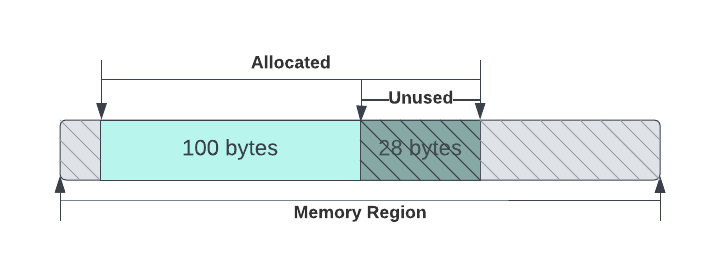
\includegraphics[width=0.75\textwidth]{figures/internal_fragmentation.png}
    \caption{A memory region containing one allocated piece of memory that is 128 bytes large. However, the user only requires 100 bytes of those and thus, 28 bytes is wasted.}
    \label{fig:internal_fragmentation}
\end{figure}

External fragmentation occurs when there is enough memory available in total but dispersed in smaller, non-contiguous chunks. This is illustrated in Figure~\ref{fig:external_fragmentation}, where a total of 80 bytes is available in total, distributed in the memory region. However, the user is unable to allocate more than 32 bytes due to the smallest uninterrupted memory chunk being only this size.

\begin{figure}[H]
    \centering
    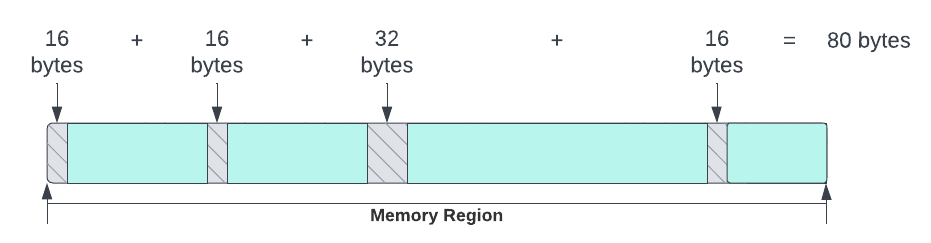
\includegraphics[width=0.8\textwidth]{figures/external_fragmentation.png}
    \caption{A memory region containing several allocated blocks with unused space in between them. Although the total sum of the unused portions is large, a request of more than 32 bytes cannot be fulfilled.}
    \label{fig:external_fragmentation}
\end{figure}

Managing and reducing fragmentation is crucial in optimising memory usage for long-running programs, as excessive fragmentation can impede the system's ability to efficiently allocate contiguous blocks of memory for new objects.

%%% Local Variables:
%%% mode: latex
%%% TeX-master: "main"
%%% End:


\subsection{Memory Allocation}
\label{sec:memory_allocation}

In this section we will describe two fundamental allocation strategies, called sequential allocation and free-list allocation, in addition to the more complex case of using multiple free-lists.

\subsubsection{Sequential Allocation}
% Describe bump-pointer/sequential/linear allocation.

Sequential allocation represents one of the most straightforward methods for allocating memory within a contiguous chunk of memory. In this approach, a pointer, often referred to as the 'bump pointer,' is used to keep track of the current position within the memory chunk. As new objects are allocated, the pointer is moved forward by the size of the object and any necessary padding or alignment. Sequential allocation is also known as 'bump-pointer allocation' due to the incremental 'bumping' of the pointer with each new allocation. It is a simple and efficient method, particularly suitable for scenarios where memory is managed linearly. Despite its simplicity, sequential allocation can be highly effective in situations where memory fragmentation is not a significant concern and where a predictable, sequential layout is desirable.

While this approach is easy to implement, it may not be the most suitable choice for all scenarios, especially in systems with varying memory demands or those requiring more sophisticated memory management strategies. Nevertheless, its simplicity makes sequential allocation a valuable technique in specific use cases.

\subsubsection{Free-List Allocation}
An alternative to sequential allocation is free-list allocation, which records the location and size of free blocks in a data structure, such as a linked list for example. In the simplest form one would use a single list for storing free blocks. An allocator would then consider each block in a sequential manner and choose one according to some policy. Below we will give an overview of how the most common policies work.

\begin{description}
    \item[First-fit]
        The first block that is large enough for satisfying a request will be used. This minimizes search time, but does not consider that there might exist a more suitable block elsewhere in the free-list. This search is restarted from the list's head for each new request. 
    \item[Next-fit]
        Searching for a block is initially done in the free-list like what is described for first-fit. In subsequent searches however, it resumes from where the previous search concluded, enhancing efficiency when searching for a new block. This approach is based on the observation that small blocks often accumulate at the start of the free-list, streamlining the search space by starting further into the list in the next iteration.
    \item[Best-fit]
        The entire free-list will be searched until the smallest available block that can satisfy a request is found. The main benefit of best-fit is that fragmentation is minimized at the cost of additional search time.
\end{description}

The three policies described above, and many others, have in common that when a block that is larger than what is requested is found, it is split up. We generally want to split block as infrequently as possible to have larger blocks available for larger request sizes. If blocks are split too often, many small blocks might accumulate, which might increase external fragmentation to a level where new requests cannot be fulfilled. Additionally, splitting blocks less frequently will also mean less merging, or coalescing, of blocks to larger sizes, which could improve performance.

\subsubsection{Segregated-Fit Allocation}
Instead of using a single free-list where blocks of many sizes are stored, one might instead use multiple free-lists that store blocks of similar sizes or size ranges, called segregated-fit. The ambition of using multiple free-lists is to narrow down the search space to fewer blocks, allowing us to find blocks large enough to satisfy a request faster. However, there is an added overhead of storing a pointer to the head of each free-list which is usually insignificant. It is crucial to note that blocks are logically segregated into their respective free-lists based on size but are not required to be physically adjacent in memory within the same free-list. This distinction emphasizes the organizational structure of segregated-fit.

Segregated-fit is often employed in real-time systems where predictable and efficient memory allocation is crucial. The reduced search space and minimized search time to find suitable blocks allows timing constraints to be met.

%%% Local Variables:
%%% mode: latex
%%% TeX-master: "main"
%%% End:


\subsection{HotSpot JVM}
\label{sec:hotspot}
\input{text/Hotspot}

\subsection{Garbage Collection}
\label{sec:gc}
As previously mentioned, garbage collection is a method of achieving automatic memory management where the system identifies and cleans up unused objects, which are considered garbage. This removes the requirement of managing memory from the user, which reduces the possibility of memory related issues occurring. This also removes some control from the user, and could lead to sub-optimal usage of system memory.

%%% Local Variables:
%%% mode: latex
%%% TeX-master: "main"
%%% End:


\subsection{The Z Garbage Collector}
\label{sec:zgc}

The following sections will cover the basics of how ZGC allocates data and how it can dynamically collect garbage. The information is based partly on an overview by A. M. Yang and T. Wrigstad~\cite{zgc:deep_dive} and partly on the source code of ZGC itself, as available in OpenJDK version 22.32~\cite{jdk:tag2232}.

%%% Local Variables:
%%% mode: latex
%%% TeX-master: "main"
%%% End:


\subsubsection{Pages}
\label{sec:zpage}

ZGC is a region-based garbage collector which allocates objects inside differently-sized regions of memory that are referred to as pages. When new objects are created, they are allocated inside pages with respect to their size. Pages are classified as one of three different types: \textit{Small}, \textit{Medium} or \textit{Large}, which support allocations of different size ranges, as specified in Table~\ref{table:zpage_sizes}. All allocations are aligned to 8 bytes and the smallest supported allocation size is, at the time of writing, 16 bytes. As a result of all allocations having the same alignment, their offset from the start of the page will also be a multiple of 8 bytes.

\begin{table}[H]
    \centering
    \begin{tabular}{lllll}
        Page Type   & Page Size     & \multicolumn{3}{l}{Object Size}      \\ \hline
        Small       & 2 MB          & \multicolumn{3}{l}{{[}16B, 256KB{]}} \\
        Medium      & 32 MB         & \multicolumn{3}{l}{(256KB, 4MB)}     \\
        Large       & $\geq$ 4 MB   & \multicolumn{3}{l}{$\geq$ 4MB}       \\
    \end{tabular}
    \caption{Page sizes in ZGC. (Figure taken from~\cite{zgc:zpage_size_table}). }
    \label{table:zpage_sizes}
\end{table}

Pages in ZGC include metadata that allows them to perform allocations efficiently, as well as ensure safe execution while running concurrently executing threads. An overview of this metadata is shown in Figure~\ref{fig:zpages}, where the most important attributes are the: \textit{Bump Pointer}, \textit{Live Map}, \textit{Sequence Number}, and \textit{Age}, which are explained in detail below.

\begin{description}
    \item[Bump Pointer]
        The bump pointer is a pointer within the page's memory range that stores the location of where new allocations are made inside the page. Its functionality and use-case are explained in detail in Section~\ref{sec:bump_pointer}. All allocations inside pages in ZGC are currently done using bump pointers. In Figure~\ref{fig:zpages}, the bump pointer is displayed below four allocated objects, indicating that the next position to allocate objects at would be below the fourth object.

    \item[Live Map]
        The live map is used to keep track of which objects are currently live and have been marked as reachable by the program. Objects not marked in the live map are considered dead. The live map is shown on the right-hand side of Figure~\ref{fig:zpages}. It is constructed during the marking phase of the GC cycle as live objects are encountered during memory traversal and marked in the live map. The live map is represented by a bitmap, where each bit is mapped to an 8-byte chunk of the page. If a bit is set, there is a live object at the corresponding address on the page. The live map is used during the compacting phase of the GC in order to know how much memory is alive inside the page.
        \newpage
    \item[Sequence Number]
        Every page has a sequence number denoting during which GC cycle it was created. If the GC is on its $N$th cycle, pages created during that GC cycle will have a sequence number $N$. Pages with sequence number $N$ are called \textit{allocating} pages, and are the only pages which allocate new objects for mutator threads. Pages with a sequence number below the current GC cycle, $0$--$N-1$ are called \textit{relocatable} pages since there will be no additional allocations done inside them during the GC cycle, and garbage can be reclaimed with the use of relocation. For example, if the current Java program has performed 5 GC cycles, any allocations after that will be exclusively done on pages with sequence number 5. If the program decides to run a 6th cycle, only garbage from pages with sequence numbers 0 through 5 will be collected, and new allocations will be done on pages with sequence number 6.

    \item[Age]
        ZGC is a generational garbage collector, meaning it treats objects of varying ages differently to improve performance. This is based on the observation that most objects survive for only a short period and those that survive for longer tend to live for a long time. ZGC applies this approach on a page-by-page basis, where all allocations on a page share the same age, which is conveniently stored on each page instead of for every object. Objects are grouped into three different age categories: \textit{Eden}, \textit{Survivor} and \textit{Old}. The \textit{Eden} age is for first-time allocation, \textit{Survivor} signifies objects that have survived one or more GC cycles and \textit{Old} those that have survived a threshold of cycles in the \textit{Survivor} age. Classifying pages this way allows the GC to treat pages of a certain age differently, which is especially useful for \textit{Eden} pages, which tend to accumulate garbage quickly.
\end{description}

\begin{figure}[H]
    \centering
    \includesvg[scale=0.8]{figures/zpage_withage.svg}
    \caption{Illustration of a page in ZGC showing what kind of metadata is kept track of to facilitate allocation and object bookkeeping. The page contains three live objects marked in green and with the corresponding bit set in the live map to the right. Red objects are previously allocated objects which have since become unreachable garbage memory.} 
    \label{fig:zpages}
\end{figure}

\subsubsection{The Garbage Collection Cycle}

Figure~\ref{fig:zgc_timeline} shows a timeline of a garbage collection cycle in ZGC, made up of an example heap and pages. The timeline shows the different phases of a cycle and how the garbage collector prepares for relocating memory to free unused memory. The three different steps in the timeline show:

\vspace*{-0.4cm}

\begin{enumerate}[label=\alph*)]
    \item The initial state of the heap before the GC cycle starts. The left page has about 30\% free memory and the right page has about 50\%. The current GC cycle is 1, which tells us that pages with sequence number 1 are allocating objects.
    \item The GC cycle has started, and the old pages have been locked. New allocations are now done on new pages instead of the old ones. The old pages are now guaranteed to not allocate any new objects, which makes it possible for the marking phase to begin to traverse the live objects.
    \item The GC has finished the marking phase and now has liveness data that indicate where live objects are allocated inside the relocatable pages.
\end{enumerate}

\vspace*{-0.4cm}

\begin{figure}[H]
    \centering
    \begin{subfigure}[t]{.214\textwidth}
        \centering
        \includesvg[width=1\textwidth]{figures/zrel1.svg}
        \caption{Initial state of the heap before the first GC cycle. The gray color indicates the page is allocating objects.}
        \label{fig:zrel1}
    \end{subfigure}
    \hfill\vline\hfill
    \begin{subfigure}[t]{.32\textwidth}
        \centering
        \includesvg[width=1\textwidth]{figures/zrel2.svg}
        \caption{The state of the heap after marking has started. The blue color indicates that the page is no longer being allocated on.}
        \label{fig:zrel2}
    \end{subfigure}
    \hfill\vline\hfill
    \begin{subfigure}[t]{.32\textwidth}
        \centering
        \includesvg[width=1\textwidth]{figures/zrel3.svg}
        \caption{The state of the heap after all live objects are marked. The red and green colors indicate that the marking phase has finished, and the pages have liveness data that explain where live objects(green) are located}.
        \label{fig:zrel3}
    \end{subfigure}
    \caption{Timeline of a garbage collection cycle, showing the state of the heap in the different phases.}
    \label{fig:zgc_timeline}
\end{figure}

\vspace*{-0.49cm}

ZGC frees memory marked as garbage by copying live objects from one page to another and re-purposing the source page for new allocations. This leads to the fragmented layout of allocated memory to be compacted which makes it possible to fit objects from multiple pages into a single one. The process of copying live objects is referred to as relocation. When performing relocation, two different scenarios can occur. Either the heap has enough free memory to allocate a new page of contiguous free memory to relocate objects to, or the heap is full, requiring the objects to be compacted into the same page that they are already located in, called in-place compaction. The first scenario is illustrated in Figure~\ref{fig:zrel_new}. This requires the heap to have enough free space available to create a new page during the time of relocation. The GC can reclaim garbage memory by relocating live objects from sparsely populated pages into a more dense configuration inside a new page. The fragmentation and also total heap usage is therefore reduced.

\begin{figure}[H]
    \centering
    \begin{subfigure}[t]{.2\textwidth}
        \centering
        \includesvg[width=1\textwidth,height=1.2885\textwidth]{figures/zrel_new1.svg}
        \caption{A page has been selected for relocation due to high fragmentation.}
        \label{fig:zrel_new1}
    \end{subfigure}
    \hfill\vline\hfill
    \begin{subfigure}[t]{.2\textwidth}
        \centering
        \includesvg[width=1\textwidth]{figures/zrel_new2.svg}
        \caption{A new page is created with a new sequence number that is used as a relocation target.}
        \label{fig:zrel_new2}
    \end{subfigure}
    \hfill\vline\hfill
    \begin{subfigure}[t]{.2\textwidth}
        \centering
        \includesvg[width=1\textwidth]{figures/zrel_new3.svg}
        \caption{The objects from the first page are relocated to the new page.}
        \label{fig:zrel_new3}
    \end{subfigure}
    \hfill\vline\hfill
    \begin{subfigure}[t]{.2\textwidth}
        \centering
        \includesvg[width=1\textwidth]{figures/zrel_new4}
        \caption{All objects have been copied to the new page and the old page is re-purposed.}
        \label{fig:zrel_new3}
    \end{subfigure}
    \caption{An example of how a successful relocation is done when the heap has enough space to allocate a new page.}
    \label{fig:zrel_new}
\end{figure}

Typically, many sparsely populated pages can be compacted onto a single new page, but this is conditional on there being enough memory to allocate the new page. Since we are starting GC as a reaction to high memory pressure, this may not always be the case. If a new page cannot be allocated, the first page is "created" by compacting its objects in-place, and then continuing by relocating the live objects of other pages onto that page. An in-place compaction is an expensive operation that re-arranges the objects of a page without a separate page as a destination. It requires the thread performing the re-arrangement to write to the memory of the page while other threads may read its contents. To do this safely, any threads trying to read from the page during this process must be paused, which removes concurrent execution of the page. The process of in-place compaction of a page is illustrated in Figure~\ref{fig:zrel_in}.

\begin{figure}[H]
    \centering
    \begin{subfigure}[t]{.2\textwidth}
        \centering
        \includesvg[width=1\textwidth,height=1.2885\textwidth]{figures/zrel_in1.svg}
        \caption{The first live object on the page is moved to the start of the page.}
        \label{fig:zrel_in1}
    \end{subfigure}
    \hfill\vline\hfill
    \begin{subfigure}[t]{.2\textwidth}
        \centering
        \includesvg[width=1\textwidth,height=1.2885\textwidth]{figures/zrel_in2.svg}
        \caption{The second live object is moved as close to the start as possible.}
        \label{fig:zrel_in1}
    \end{subfigure}
    \hfill\vline\hfill
    \begin{subfigure}[t]{.2\textwidth}
        \centering
        \includesvg[width=1\textwidth,height=1.2885\textwidth]{figures/zrel_in3.svg}
        \caption{All objects have been moved, and the space after is made available.}
        \label{fig:zrel_in1}
    \end{subfigure}
    \hfill\vline\hfill
    \begin{subfigure}[t]{.2\textwidth}
        \centering
        \includesvg[width=1\textwidth,height=1.2885\textwidth]{figures/zrel_in4.svg}
        \caption{The bump pointer is moved to the beginning of available space.}
        \label{fig:zrel_in1}
    \end{subfigure}
    \caption{An example of how in-place compaction is done to remove fragmentation.}
    \label{fig:zrel_in}
\end{figure}
 
%%% Local Variables:
%%% mode: latex
%%% TeX-master: "main"
%%% End:


\section{Related work}

% I want to describe that even though allocators have been designed about for a long time, the problem is still not solved.
% Perhaps quote the TLSF paper?

Due to the large number of existing allocator designs, one might draw the conclusion that most problems of dynamic memory allocation have already been solved. For most cases, a general purpose allocator designed to be used in any system or environment performs well on average, in terms of response time and fragmentation. However, there often exist areas of improvement depending on how much the use case is narrowed down. For example, a garbage collector using an allocator know more about the objects being allocated than most other users of an allocator would.

From the widely used dlmalloc by Doug Lea~\cite{dlmalloc} and newer adaptations of it such as jemalloc and tcmalloc

One of the most widely used allocators is dlmalloc, created by Doug Lea~\cite{dlmalloc}. 

%%% Local Variables:
%%% mode: latex
%%% TeX-master: "main"
%%% End:


\section{Two-Level Segregated Fit}
\label{sec:tlsf}

Two-Level Segregated Fit (TLSF) is a dynamic storage allocator by Masmano et al.~\cite{TLSF}. It is especially designed to be used in real-time applications, where it stands out among other allocators in that it has a bounded and short response time and maintains low fragmentation, thus ensuring high predictability. 

\subsection{Allocation and Freeing Strategy}

From the perspective of the user, TLSF has the same interface as \texttt{malloc()} and \texttt{free()} in libc~\cite{mallocman}. What makes TLSF unique is its internal mechanisms, which are discussed next.

When the user requests N bytes from the allocator, the allocator aligns N to meet any necessary alignment requirements and applies padding. Subsequently, it checks the free-list matching the allocation request to see if it contains any block(s). If no block is found in the list, the allocator checks if any free-list contains blocks larger than the requested size. If no list containing large enough blocks is found, NULL is returned. However, if a list containing block(s) of large enough size is found, the allocator removes the first block in the list, regardless of the number of blocks in it. The policy of searching for free-lists and choosing the first block is called Good-Fit by the authors, referred to as a combination of best- and first-fit. Good-Fit performs well in that search times are low and block sizes often align with the allocation request, requiring little to no additional overhead. Moreover, if a block larger than the requested size is located, the allocator splits it into two blocks. One block is used to satisfy the request to the user, and the other is inserted back into the allocator. Figure~\ref{fig:tlsf_allocation} shows this process.

\begin{figure}[h]
    \centering
    \includesvg[width=1.0\textwidth]{figures/tlsf_allocation.svg}
    \caption{The process of allocating memory in the TLSF allocator.}
    \label{fig:tlsf_allocation}
\end{figure}

When a block is freed, TLSF tries to coalesce the block with its neighboring blocks if they are free. Immediately coalescing when freeing allows the allocator to have larger blocks available for larger request sizes as often as possible. Having as few small blocks as possible minimizes fragmentation. After coalescing has been attempted, the block is inserted into the free-list matching its final size.

\subsection{Technical Description}

The name Two-Level Segregated Fit reflects its design as a free-list-based allocator that uses segregated-fit, storing multiple free-lists containing blocks of set size classes. To efficiently lookup what free-list are non-empty, TLSF employs two levels of bitmaps. A first-level bitmap for size classes that are separated by powers of two and a second-level bitmap that subdivides the first-level size classes linearly. In the reference implementation, the number of first- and second-levels is limited to 32 in order to fit in 32 bits. Additionally, the number of second-levels is recommended to be a power of two for efficiency reasons, so that simple bit-shift instructions can be used. The combined use of multiple free-lists and bitmaps for information bookkeeping enables the asymptotic worst-case response times for allocating and freeing memory to be constant, i.e. \texttt{O(1)}, since it limits the number of instructions for finding blocks.

Allocations inside TLSF are managed using blocks. Blocks are kept track of in two doubly-linked list structures. Initially, blocks are arranged in a physically ordered list by their place in memory, and if a block becomes free, it is then inserted into an appropriate free-list, that is ordered by block size instead. Each block is accompanied by an associated header located next to it. The header specifies the size of the block and also its position within both doubly-linked lists and contains different data depending on whether it is free or not. Free blocks contain additional data over allocated blocks, as shown in Figure~\ref{fig:blockheader_reference}.

Moreover, block sizes are aligned to multiples of the allocation unit (4 bytes for a 32-bit architecture). The two least significant bits within the block header are reserved for metadata. These bits indicate whether the block is free (F-bit) and whether it represents the last block within its pool (L-bit), as depicted in Figure~\ref{fig:blockheader_reference}. The F-bit is mainly used to see whether a block can be coalesced, and the L-bit to easily iterate over physical blocks.

The TLSF authors primarily focus on low-level allocation primitives without explicit consideration for garbage collection. Consequently, exploring the adaptation of TLSF to integrate with a garbage collector represents a direction for advancing its development, which is the main focus of this work.

\begin{figure}[H]
    \centering
    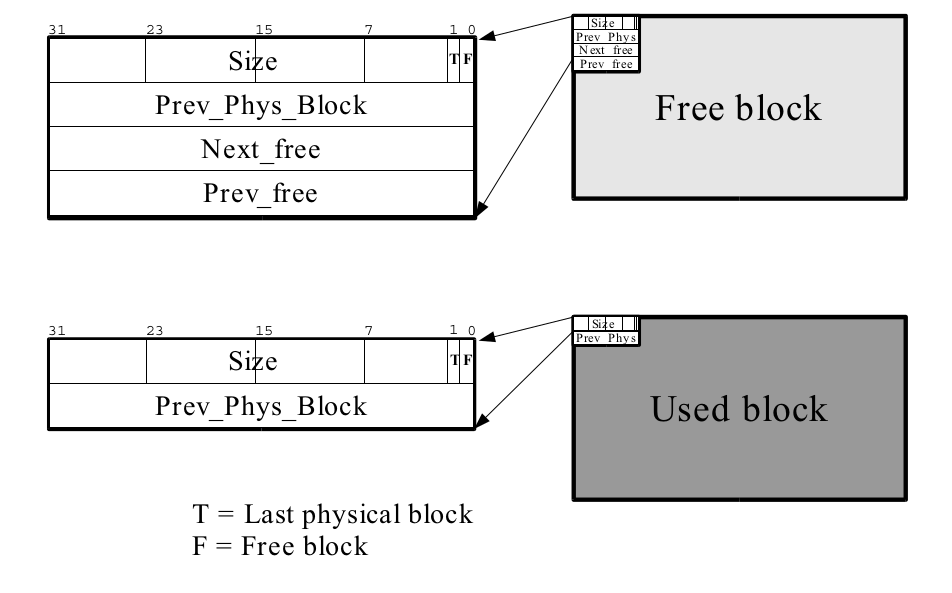
\includegraphics[width=0.80\textwidth]{figures/blockheader_reference.png}
    \caption{Representation of free and allocated block headers in 32-bit architecture. For a 64-bit architecture, each field is 8 bytes instead of 4 bytes (Taken from Masmano et al.~\cite{TLSF}).}
    \label{fig:blockheader_reference}
\end{figure}

%%% Local Variables:
%%% mode: latex
%%% TeX-master: "main"
%%% End:


\section{Method}
\label{sec:method}

The methodology is divided into four distinct phases:

\begin{enumerate}
    \item Implement a reference version of an allocator and verify its functionality.
    \item Identify important aspects for memory allocation in garbage collection.
    \item Adapt the reference version with regard to aspects from previous step.
    \item Evaluate the adaptations and how they compare to the reference version.
\end{enumerate}

The initial step involves implementing a reference version of the TLSF memory allocator, that can be used as a starting ground for adaptations. Additionally, having a reference implementation helps in assessing the impacts of modifications more accurately. The functionality of the reference implementation is verified using real-world programs, which entails substituting \texttt{malloc()} and \texttt{free()} with a wrapper that utilizes the reference version of the allocator. 

Substitution is done using the \texttt{LD\_PRELOAD} environment variable in Linux, which enables the preloading of shared libraries prior to system libraries, allowing us to use our allocator instead of the one provided by the system. The set of specific programs that will be used for verification are commonly used Linux-programs: \texttt{cat}, \texttt{grep}, \texttt{ls}, \texttt{nano}, \texttt{sed} and \texttt{wc}. It would be optimal to verify functionality on more programs. However, extensively testing a memory allocator is both a time and resource intensive process. Instead, we focus on making sure the allocator works on this subset of programs, which will later be used to evaluate adapted versions of the allocator as well. The reference version is considered working if it successfully manages to allocate memory for these programs and does not crash during runtime.

The next step is identifying important aspects related to memory allocation within the context of garbage collection. This is essential for making informed decisions during the adaptation process. By identifying key aspects, we are able to gain insight into areas where improvements are likely to have significant impact, and are thus most valuable in spending time on. Finding aspects will mainly be done through literature review in the area of memory allocation and garbage collection, as well as insights about ZGC and general memory usage patterns in Java programs. The findings from this step will answer what boundaries are present in the context of allocating memory in ZGC and will guide us through adaptation.

Building upon the insights gained from the previous step, the reference implementation is adapted in areas which are likely to be beneficial for one of or both performance and memory efficiency. The adaptation process is conducted incrementally, with each modification being tested through unit tests to ensure that the allocator behaves as intended in every step, which helps in ensuring that adaptations are purposeful and aligned with the research objectives. 

Finally, both the reference implementation and its adapted version(s) will be compared in terms of their performance and memory efficiency. This along with the adaptations that are made to the allocator will answer the second research question regarding how the boundaries can be utilized to improve the allocator. More on specific metrics, evaluation method and steps to reproduce in Section~\ref{sec:evaluation}.

%%% Local Variables:
%%% mode: latex
%%% TeX-master: "main"
%%% End:


\section{Allocator Adaptations}
\label{sec:adaptations}
In this section we describe the adaptations that have been made to the reference implementation of TLSF to make it more suited toward being used in the context of a garbage collector, specifically ZGC.

\subsection{Architectural Considerations}

ZGC is solely implemented for 64-bit architecture and does not support 32-bit~\cite{zgc_deep_dive}. Hence, in our effort to adapt the allocator for ZGC, it is reasonable for the allocator to also be limited to the same scope. The authors of TLSF have designed their allocator primarily for 32-bit systems due to it being targeted toward real-time embedded systems, which usually operate on 32-bit architecture. However, while TLSF was initially designed with 32-bit systems in mind, its design principles and concepts are not inherently tied to any specific architecture. Hence, adapting the allocator to 64-bit systems does not require any significant changes in its design, apart from aligning memory toward the allocation unit of 8 bytes for 64-bit systems instead of 4 bytes for 32-bit systems.

\subsection{General and Optimized Versions}

When adapting the allocator we will consider the use cases of either using it as a normal allocator in cases where a traditional malloc/free combination is used, or as a way to allocate objects on pages in ZGC. To minimize the codebase, which is desirable from a maintenance perspective, the allocator will be adapted in a way which allows it to be configured for different use-case. A major benefit of doing this is that different configurations can easily be compared against each other, streamlining the process of measuring efficacy of any adaptations that are made.

Worth noting however, is that in the process of redesigning the allocator in a configurable manner, some changes that deviates from the reference implementation will have to be made. Such trade-offs, which will be discussed in more detail later, could be reasonable when extending the interface for supporting multiple configurations, or versions, of the allocator.

\subsection{Reduced Allocation Size Range}

In ZGC, small and medium pages only allow the user to allocate in certain size ranges. To our advantage, we can use this to store metadata about the allocator in a more efficient way. Small pages allow sizes in the range [16B, 256KB] and medium pages (256KB, 4MB]. We note that the allowed sizes in the medium range is a factor of 16KB larger than the small range. This allows us to limit the allocator to the size range of small page, with an additional multiplication factor of 1 for small pages and 16KB for medium pages.

With the limited allocation size range for small pages in mind, we are able to limit the number of free-lists we need and in turn the bits used in the bitmaps. We need 14 first-levels to be able to index every power of two inside the small page range, with a lower-bound of $2^4 =$ 16B and an upper-bound of $2^{17} =$ 128KB. It is desirable to store all bitmap information in a single 64-bit word for performance reasons, both in terms of cache efficiency and usage of efficient bit instructions. If we want to stay inside the 64-bit limit, we must choose the number of second-levels accordingly. For efficiency reasons again, the number of second levels should be a power of two~\cite{TLSF} so that bit-shift instructions can be used. The only value this leaves us is 4, which requires $14 * 4 =$ 56 bits for storing all metadata.

Since a page is initially 2MB large, the initial block will be significantly larger than the maximum allocation size of 256KB. This means we either need to split it up into multiple blocks of smaller sizes or store it in a different free-list. To solve this we will add a last free-list that is called the "large-list", represented by the 57th bit. The large-list will store blocks that are above the largest index to support storing blocks that are initially very large.

Combining the insight of the number of required first- and second-levels, desire to use a single 64-bit bitmap and large-list, we can construct a new bitmap representation, as shown in Figure~\ref{fig:bitmap_flattening}. The new bitmap disregards the literal notion of ``Two Level'' from Two Level Segregated Fit and flattens the first- and second-level bitmaps to a single bitmap. The new bitmap is indexed using the formula: 
\[
    \text{bitmap\_index($f, s$)} = f * 4 + s
\]
where $f$ and $s$ are the first- and second-level indexes respectively. Additionally, the lowest size classes have been placed at the least significant bits of the bitmap to make searching for the next non-empty free-list efficient using the find-first-set bit instruction.

\begin{figure}[H]
    \centering
    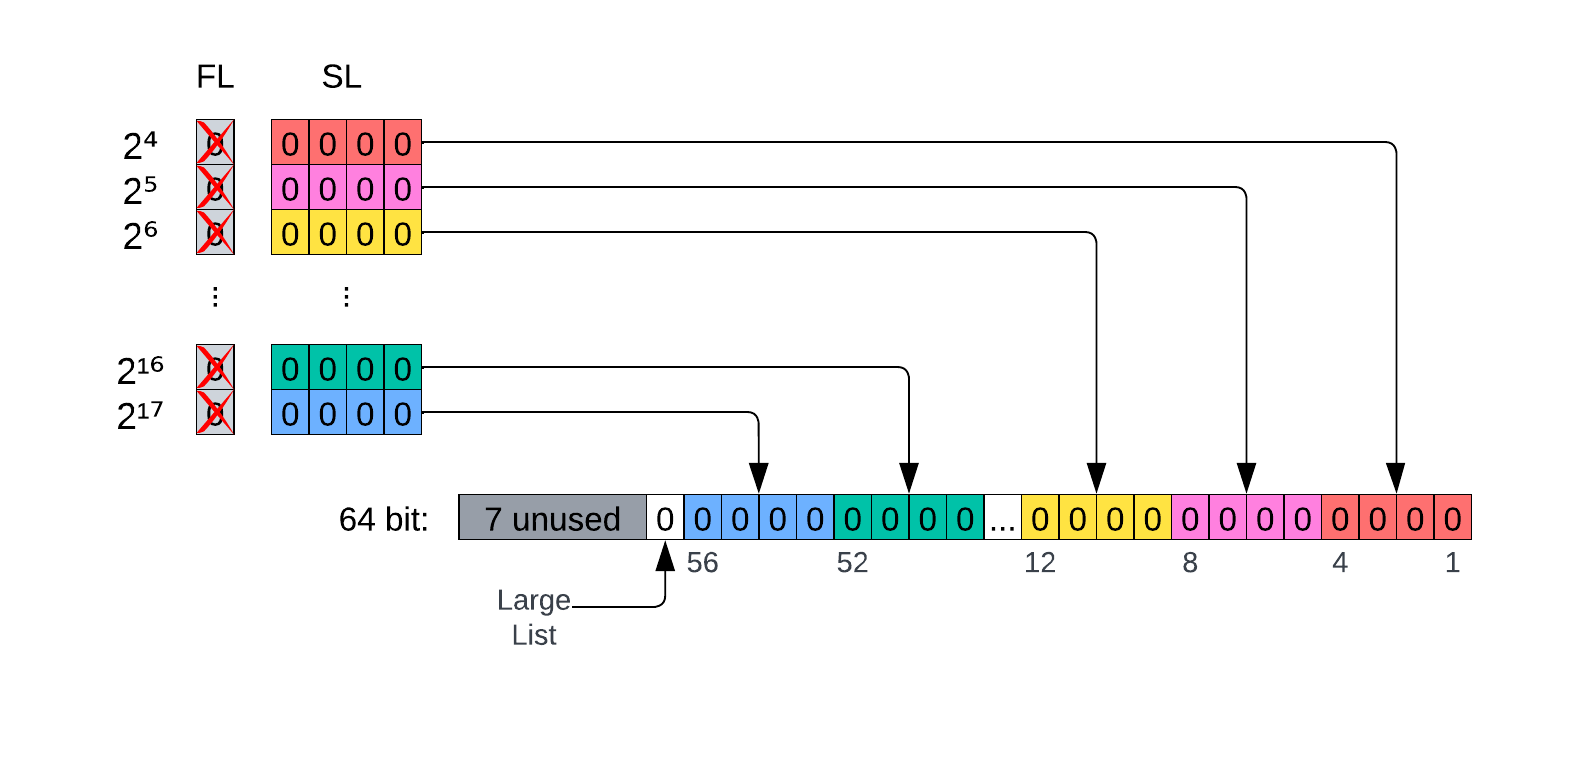
\includegraphics[width=1\textwidth]{figures/bitmap_flattening.png}
    \caption{Flattening of the 2D-matrix representation of TLSF bitmaps into a single 64-bit value. The first-level bitmap is disregarded in favor of indexing the new flattened bitmap using the first-level value instead. The number of first-levels are 14, indicated by bits of the same color belonging to the same first-level. The number of second-levels are 4, as indicated by the same number of colored bits.}
    \label{fig:bitmap_flattening}
\end{figure}

The correlation between the bitmap and the free-lists is depicted in Figure~\ref{fig:bitmap_relationship}, adhering closely to the original TLSF design. However, the adaptation now efficiently determines the relevant free-list by looking in the single bitmap, not two bitmaps as in the original design.

\begin{figure}[H]
    \centering
    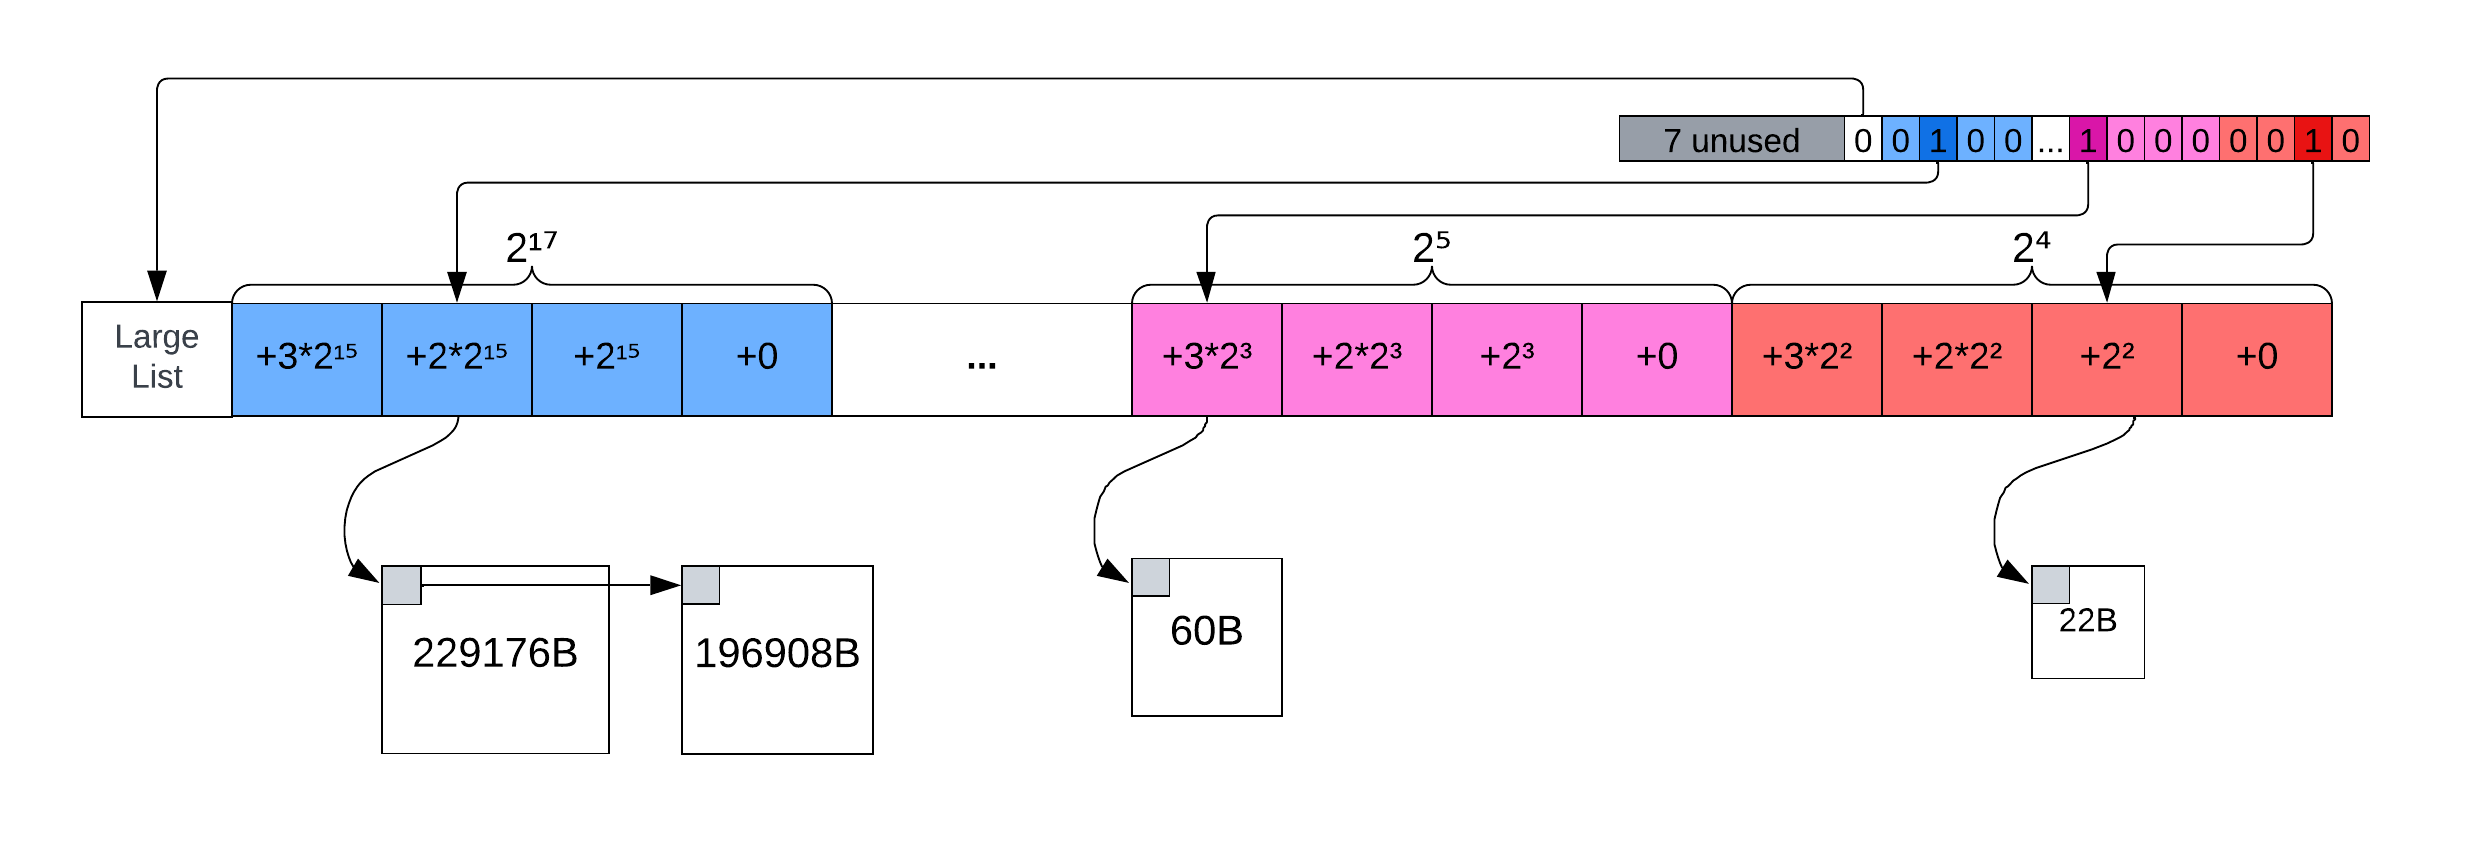
\includegraphics[width=1\textwidth]{figures/bitmap_relationship.png}
    \caption{Relationship between the new bitmap representation and accessing the corresponding free-lists.}
    \label{fig:bitmap_relationship}
\end{figure}

% TODO: Detta borde flyttas till discussion.
% A drawback of dividing the memory into only four second-levels per fist-level is that there is less chance that a block is closer to the size that we want to allocate. This could potentially lead to higher fragmentation, as there are fewer size classes of blocks available. However, this is generally not a problem...

% TODO: Cite TLSF paper.
% Benefits: Reduced memory overhead, cache efficiency, Simplified indexing (and Atomic operations??)
% Drawbacks: Reduce number of second-level partitions to 4, instead of more, which could have an impact on internal fragmentation.

\subsection{Transitioning Between Different Allocation Strategies}

Completely phasing out the utilization of bump-pointer allocation may not be optimal, especially when there is no constant requirement to allocate solely within the ``holes'' of a page. Instead, users could employ bump-pointer allocation up to a certain point, at which it becomes advantageous to transition to a more sophisticated allocator for non-bump-pointer allocation.

Most allocators start with an unused chunk of memory, allowing them to track and keep an up-to-date record of what the underlying memory contains. However, in the case where transitioning from bump-pointer to using an allocator, the underlying memory have contents that is not represented in the allocator. To solve this, we need to update the allocator's internal representation to align with the contents of the memory. In ZGC, the latest live analysis of a page contains an accurate representation of what data is alive in the page's underlying memory. This information can therefore be used to update the allocator's internal representation after a transition to using an allocator.

The construction of the allocator's representation involves a two-step process that extends the optimized allocator's API. Initially, the representation must be cleared so that any previous data is removed. When clearing the allocator, a block is allocated to cover the entirety of the underlying memory. This allows the user to invoke a function to free blocks within specified ranges, allowing to selectively ``carve'' segments free memory from the initially allocated block. When freeing ranges of memory, we only consider four cases: 

\begin{enumerate}
    \item The range is strictly within an allocated block and does not start nor end on the block's edges.
    \item The range begins at the start of the block and ends on the end of the block.
    \item The range starts inside the block and ends on the block's end.
    \item The range starts at the block's start and ends inside the block.
\end{enumerate}

We will not consider cases where the range overlaps multiple blocks and start or end on the edge of a block that is not the last or the first block in the physical order. This is because if a user wants to free a consecutive range of 64 bytes for example, they should always free the entire 64 byte range directly and not the first 32 bytes followed by the next 32 bytes. This reduces complexity of the implementation without significantly impacting user functionality.

\subsection{Deferred Coalescing of Blocks}

In the process of allocating and freeing blocks within an allocator, the general preference is to always have as large blocks as possible available to fulfill larger requests. However, in scenarios where numerous small allocations are frequently made and free'd, the emphasis on coalescing blocks to accommodate larger requests in the future may not be worthwhile. Instead, coalescing of blocks will be deferred until a later point in time or none at all.

The idea behind deferred coalescing is that when the user calls free(), the block being freed is not implicitly attempted to be coalesced with its adjacent physical neighbors. Instead, the allocator's API is extended to include an explicit coalesce operation. This operation scans through all blocks and coalesces as many as possible. Unlike immediate coalescing, this deferred approach postpones the process until a later point when a larger block is required.

The explicit coalesce operation conducts a pass over all blocks, requiring only knowledge of the size of the current block to identify the location of the next block. This eliminates the need to store a pointer to the physical neighbor right before the current block, which is only used when coalescing in a free() call. The algorithm describing how the pass is done is shown in Algorithm~\ref{algorithm:coalesce_blocks}.

\begin{algorithm}[H]
current = first\_physical\_block\\
\While{current != nullptr} {
next = get\_next\_block(current)\;
\uIf{next != nullptr \textbf{and} current->is\_free() \textbf{and} next->is\_free()} {
    current = coalesce\_neighbors(current, next)\;
    insert\_block(current)\;
}
\Else {
    current = next
}
}
\label{algorithm:coalesce_blocks}
\caption{Algorithm for explicitly coalescing all possible free blocks in the allocator. Note that coalesce\_neighbors() removes both blocks from the free-list before the newly coalesced block is inserted.}
\end{algorithm}

\subsubsection{Disregarding Size for Allocated Blocks}

\subsubsection{Block Header Adjustments}

R. Jones et al~\cite[Page 103]{gchandbook} discuss that in the context of using allocators in garbage collectors, it is a reasonable approach to remove certain parts of the so called boundary tag, or block header for TLSF. This is because a garbage collector know significantly more about the memory being processed than what a traditional system using a general purpose memory allocator does. This allows us to, for example, defer coalescing by default, transition between different allocators and optimize the bitmap layout from knowing what sizes will be allocated beforehand.

Combining the insights from the adaptations made so far, we can observe that storing a pointer to the previous physical block is no longer needed in the optimized version. This is because the previous physical pointer is only used when calling free and coalescing blocks with their physical neighbors. Following this, we will redesign the header for the previous physical pointer to be removed in the optimized version and still kept in the general version. 

% TODO: Disadventageous for small allocations, will have to be measured in practice.

The block header, as used in the reference implementation, is shown in Figure~\ref{fig:blockheader_adap_reference}. Here, the next and prev pointers are stored in the unused parts of free blocks and are unused in allocated blocks. In contrast, Figure~\ref{fig:blockheader_adap_general} shows the adapted block header for the general version of the allocator. In this version, all four fields are used for both free and allocated blocks since the previous physical pointer has been rearranged to the end of the header. Rearranging the previous physical pointer allows us to get the block header for optimized blocks, as shown in Figure~\ref{fig:blockheader_adap_optimized}. In the optimized header, the next and prev pointers have been converted to offsets, allowing them to be 32-bits each. Additionally, both the size and the now next/prev offsets are only stored in the unused parts of free blocks, allowing for a 0-byte header for allocated blocks.

% In the optimized header, the only constant overhead is the size field, as the next and prev pointers are only used in the unused parts of free blocks, as in the reference implementation. Additionally, the previous physical pointer is completely ignored in the optimized header.

\begin{figure}[H]
    \centering
    \begin{subfigure}[b]{0.3\textwidth}
        \centering
        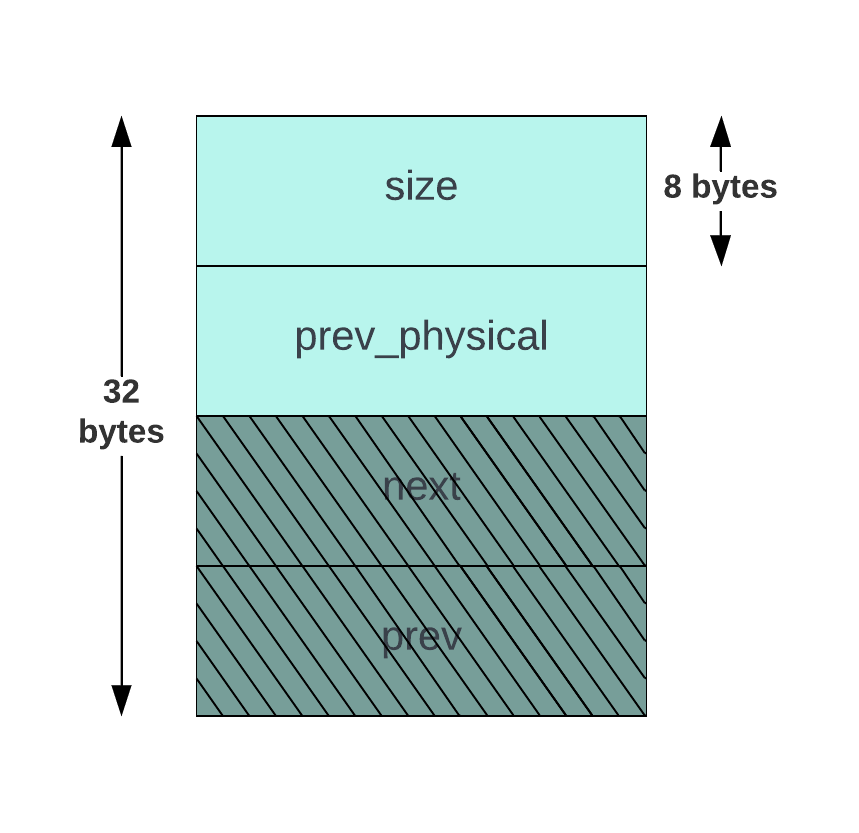
\includegraphics[width=\textwidth]{figures/blockheader_adap_reference.png}
        \caption{Reference implementation block header.}
        \label{fig:blockheader_adap_reference}
    \end{subfigure}%
    \hfill
    \begin{subfigure}[b]{0.3\textwidth}
        \centering
        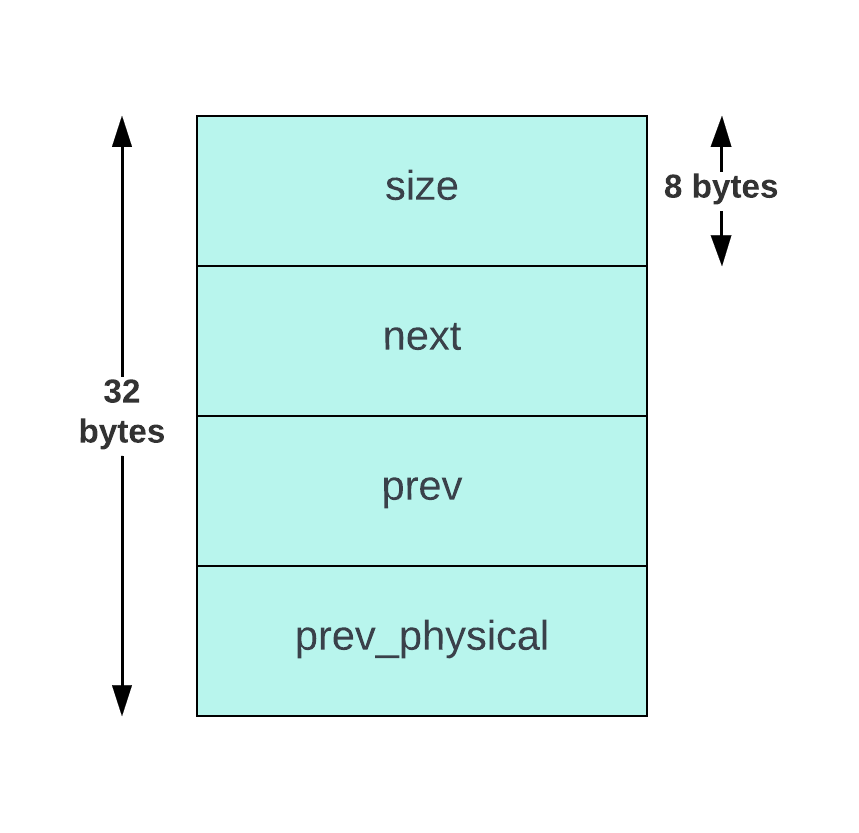
\includegraphics[width=\textwidth]{figures/blockheader_adap_general.png}
        \caption{Adapted general block header.}
        \label{fig:blockheader_adap_general}
    \end{subfigure}%
    \hfill
    \begin{subfigure}[b]{0.3\textwidth}
        \centering
        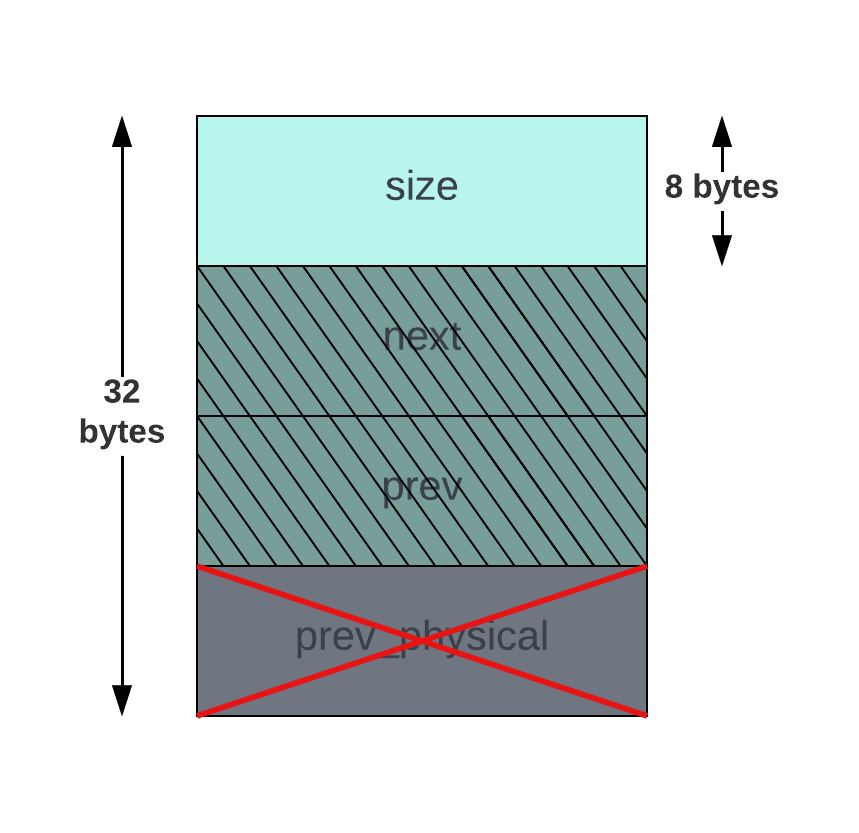
\includegraphics[width=\textwidth]{figures/blockheader_adap_optimized.png}
        \caption{Adapted optimized block header.}
        \label{fig:blockheader_adap_optimized}
    \end{subfigure}
    \caption{Overview of block header contents and adaptations. Dashed fields are only unused in the unused part of free blocks and crossed out fields are unused.}
    \label{fig:blockheader_adaptations}
\end{figure}

The goal of changing the header is to reduce the constant block header overhead required when allocating blocks. This is especially important when most allocations are small, where the block overhead is most significant. With the new design for the block header, the constant block header overhead for the optimized version is reduced to only 8 bytes for storing the size of the block. However, reducing the overhead for optimized headers has required us to instead increase the overhead for the general version.

% Block sizes can be stored in much less than 64 bits, but due to alignment etc it is reasonable to use a 64-bit value to store the size anyways.

%%% Local Variables:
%%% mode: latex
%%% TeX-master: "main"
%%% End:
=======
\subsection{Lazy Layer}
Lazy list description

\subsection{Inverse Order}

Inverse free-list traversal (ibuddy / restructure of metadata)


\subsection{Allocator Regions}
Split allocator into regions


\subsection{Determining Size}

Reduce the size bits needed (removed in future??)


\section{Implementation Details}
\label{sec:adaptations-impl}

This section provides the implementation specifics for the adaptations described in the previous section, focusing on those that require detailed explanation. It covers the technical aspects and modifications necessary to optimize the TLSF allocator for use with ZGC.

\subsection{Allocator Configurations}

The reference implementation of the allocator has been abstracted into a base class named \texttt{TLSFBase}. From the base class, the user must provide a set of configuration variables that define how the allocator behaves, where each unique set of configuration variables defines a new allocator. An allocator may override the implementation of the methods defined in the base class so that computations may be done differently. For example, this allows different versions to apply different allocation, freeing, and concurrency methods. The configuration variables are:

\begin{enumerate}
    \item Number of first- and second-levels (Sets the size range granularity and number of free-list)
    \item Minimum block size (The minimum size of blocks)
    \item Block header size (The size of the block header. Depends on what fields/bytes are used in the header)
    \item Usage of second-levels (When not using second-levels, the new bitmap design is used, as described in Section~\ref{sec:adaptations_impl:bitmap_design}, otherwise the reference implementation is used)
    \item Usage of deferred coalescing (Deferred coalescing disables immediate coalescing. Coalescing can only be done through explicit coalescing)
\end{enumerate}

\subsection{New Bitmap Design}
\label{sec:adaptations_impl:bitmap_design}

Summarizing the insight from Section~\ref{sec:adaptations:reduced_allocation_range} regarding the number of required first- and second-levels, the desire to use a single 64-bit bitmap and large-list, a new representation for the bitmap is constructed, as shown in Figure~\ref{fig:bitmap_flattening}. The new bitmap disregards the literal notion of ``two-level'' from Two-Level Segregated Fit and flattens the first- and second-level bitmaps to a single bitmap. The mapping for the bitmap is calculated by combining the first- and second-level mappings, which are calculated the same way as in the reference design. Hence, the mapping for the new bitmap is calculated using the formula below, where $f$ and $s$ are the first- and second-level indexes, respectively.
\[
    I(f, s) = 4f + s
\]

Like is done in the reference design, the new bitmap places the classes of the lowest size at the least significant bits to make searching for the next non-empty free-list efficient using the find-first-set (\texttt{ffs}) bit instruction. Furthermore, the new design only requires searching a single bitmap, making a single \texttt{ffs} instruction enough to find free-lists in any first-level, unlike the reference design, which requires two \texttt{ffs} instructions.

\begin{figure}[h]
    \centering
    \includesvg[width=0.8\textwidth]{figures/bitmap_flattening.svg}
    \vspace*{4mm}
    \caption{Flattening of the 2D-matrix representation of TLSF bitmaps into a single 64-bit value. The first-level bitmap is disregarded in favor of indexing the new flattened bitmap using the first-level value instead. The number of first-levels is 14, indicated by bits of the same color belonging to the same first-level. The number of second-levels is 4, as indicated by the same number of colored bits.}
    \label{fig:bitmap_flattening}
\end{figure}

The correlation between the new bitmap and free-lists is depicted in Figure~\ref{fig:bitmap_relationship}, adhering closely to the original TLSF design. The highest granularity of free-list size ranges is found for the smallest allocations, which aligns well with most allocations being small inside most Java programs. This leads to less memory potentially being wasted and less splitting done since more blocks match the request size, thus saving performance.

\begin{figure}[h]
    \centering
    \vspace*{0.2cm}
    \includesvg[width=1.0\textwidth]{figures/bitmap_relationship.svg}
    \vspace*{1mm}
    \caption{Relationship between the new bitmap representation and accessing the corresponding free-lists.}
    \label{fig:bitmap_relationship}
\end{figure}

\subsection{Block Header Adjustments and 0-byte Header}
\label{sec:adaptations_impl:0-byte-header}

The block header, as designed in the reference implementation, is shown in Figure~\ref{fig:blockheader_adap_reference}. Here, the size and previous physical pointer (prev\_phys) are constant, and the next and prev pointers are only used in the unused part of free blocks and unused for allocated blocks. In contrast, Figure~\ref{fig:blockheader_adap_general} shows the adapted block header for the general version of the allocator. In this version, all four fields are used for both free and allocated blocks since the previous physical pointer has been rearranged to the end of the header. Rearranging the previous physical pointer to be the last field in the header, as shown in Figure~\ref{fig:blockheader_adap_optimized}, makes it possible to have the same definition for the general and optimized versions, while the optimized version only uses the first 16 bytes of it.

\begin{figure}[h]
    \centering
    \begin{subfigure}[b]{0.3\textwidth}
        \centering
        \includesvg[width=\textwidth]{figures/blockheader_adap_reference.svg}
        \caption{Reference implementation block header.}
        \label{fig:blockheader_adap_reference}
    \end{subfigure}%
    \hfill
    \begin{subfigure}[b]{0.3\textwidth}
        \centering
        \includesvg[width=\textwidth]{figures/blockheader_adap_general.svg}
        \caption{Adapted general block header.}
        \label{fig:blockheader_adap_general}
    \end{subfigure}%
    \hfill
    \begin{subfigure}[b]{0.3\textwidth}
        \centering
        \includesvg[width=\textwidth]{figures/blockheader_adap_optimized.svg}
        \caption{Adapted optimized block header.}
        \label{fig:blockheader_adap_optimized}
    \end{subfigure}
    \caption{Overview of block header contents. Striped fields are only present in the unused part of free blocks and crossed-out fields are unused.}
    \label{fig:blockheader_adaptations}
\end{figure}

As stated in Section~\ref{sec:adaptations:block-header-adjustments}, the size field can be ignored for allocated blocks if the block size is kept track of somewhere else and is provided upon calling \texttt{free()}. The benefit of doing this is that more memory is available for object allocation inside ZGC pages. Consequently, this means that the size must be fetched and perhaps computed from elsewhere, adding extra operations that might decrease performance. 

Additionally, to further minimize footprint, the next and prev pointers have been converted to offsets in the optimized version, allowing them to be 32 bits each. The conversion to and from offsets and pointers means adding extra operations, which might decrease performance further at the cost of memory efficiency. The next and prev fields are only used inside the unused memory of free blocks. Neither field is used for allocated blocks, which, in addition to not storing the size of the block, requires no header at all, hence the name \textit{0-byte header}.

In summary, the increase in available memory when applying block header optimization is at the cost of potentially decreased performance and is most likely a trade-off worth making. This is because most allocations in Java are small, which results in the size of the block header taking up proportionally more memory.

\subsection{Concurrency Implementation}
\label{sec:adaptations_impl:concurrency}

Implementing concurrency for the allocator will require being able to concurrently operate on its free-lists. The free-lists, in combination with the bitmaps that store data about them, are the critical sections of the allocator. In the reference design, the free-lists are designed as doubly linked lists. However, lock-free operations on a doubly linked list will not be considered due to the complex operations required to support them. Instead, the appearance of the free-lists is simplified to make it easier to support concurrent operations.

By disregarding the pointer to the previous free block inside block headers, the appearance of the free-lists can be transformed from a doubly linked list to a singly linked list. This transformation is possible when not coalescing immediately, since the previous pointer is only used when inserting and removing blocks at positions other than the head of a free-list. Consequently, by only allowing updates at the head of a free-list, the singly linked list effectively becomes a stack, simplifying the implementation of a lock-free solution.

M. Herlihy and N. Shavit~\cite[Chapter 11]{artofmpprogramming} describe the design and inner workings of a lock-free stack on which the concurrent implementation of the allocator is largely based. For reference, a general overview of how a lock-free stack works and how it connects to the free-lists inside the allocator is described.

A stack only requires two operations: \texttt{push()} and \texttt{pop()}, which are named \texttt{insert()} and \texttt{remove()} in the allocator to stay consistent with their meaning from the general version. The insert operation replaces the head of the stack, or free-list, with a new block, while the remove operation removes the head of the free-list and replaces it with the next block, if any, in the free-list. In order to make the allocator work in a thread-safe manner, only these two operations need to be concurrent, since all other operations in the allocator can be done independently of other threads.

The free-lists will be operated on concurrently without locks using the atomic operations \texttt{load()}\footnote{\url{https://en.cppreference.com/w/cpp/atomic/atomic/load}} and \texttt{compare\_exchange()}\footnote{\url{https://en.cppreference.com/w/cpp/atomic/atomic/compare_exchange}}, provided in the C++ standard library. \texttt{load()} returns the current value of an atomic variable, and \texttt{compare\_exchange()} compares the value of a variable with an expected value, and if they are equal, it is replaced by another value.

\subsubsection{Solving The ABA Problem}
\label{sec:adaptations_impl:aba_problem}

The ABA problem occurs when a thread employs compare-and-exchange to read a value it intends to change, gets interrupted, and, upon resuming, finds the value it initially read remains unchanged, despite potential modifications by other threads. This can lead to successfully performing a compare-and-exchange operation even when modifications during the interruption could have occurred.

A strategy for solving the ABA problems is to ensure that all values, or pointers in the allocator, are inherently unique and used only once. This approach enables the detection of changes during thread preemption. However, pointers to blocks are not unique in the allocator and can be inserted and removed any number of times. One way to achieve pointer uniqueness is to apply a so-called version tag to each pointer, which makes it possible to uniquely identify pointers.

Version tagging is described by D. Dechev et al.~\cite{bjarne_aba} as a common and effective solution for the ABA problem. However, due to how compare-and-exchange works, it is desirable to store the pointer and version tag in a single word, i.e., 8 bytes on a 64-bit system. 

When using the allocator for pages in ZGC, this is not a problem, as the same principles applied in Section~\ref{sec:adaptations_impl:0-byte-header} can be used to convert 64-bit pointers to 32-bit offsets. This conversion allows storing the version tag in the remaining 32 bits of the word, as illustrated in Figure~\ref{fig:concurrent_head_bits}.

\begin{figure}[h]
    \centering
    \vspace*{4mm}
    \includesvg[width=1\textwidth]{figures/concurrent_head_bits.svg}
    \caption{Bit representation of a free-list head in the allocator. The 32 most significant bits are used to store the offset and the 32 least significant bits are used to store the version tag.}
    \label{fig:concurrent_head_bits}
\end{figure}

\subsubsection{Insertion and Removal of Blocks}

The process of concurrently inserting a block into a free-list is outlined in Listing~\ref{algorithm:concurrent_insert_block}. Between loading the old head from the free-list and executing the \texttt{compare\_exchange()} operation, the new head must be constructed using data from the old head. However, there is a potential issue wherein the thread responsible for construction may be preempted, allowing another thread to modify the head during this time. To address this, if the \texttt{compare\_exchange()} operation fails, the thread will loop and create a new head until it is successfully performed.

\begin{lstlisting}[language=C++, caption={Concurrent insertion of a lock into the head of a free-list.}, label={algorithm:concurrent_insert_block}]
void insert_block(BlockHeader blk) {
    Mapping mapping = get_mapping(blk.size);

    do {
        TaggedBlockHeader old_head = blocks[mapping].load();
        TaggedBlockHeader new_head = construct_head(old_head);
    } while(blocks[mapping].compare_exchange(old_head, new_head));

    update_bitmap(mapping);
}
\end{lstlisting}

The process of concurrently removing a block from a free-list, as illustrated in Listing~\ref{algorithm:concurrent_remove_block}, is similarly defined to block insertion. If the \texttt{compare\_exchange()} operation fails when removing a block, there is no guarantee that the same free-list contains additional blocks. In cases where thread preemption occurs during removal, other threads might exhaust the free-list, which will make further operations fail. To solve this, \texttt{remove\_block()} either succeeds or fails without looping until successfully performing a swap, like \texttt{insert\_block()} does. Consequently, the caller must recalculate the mapping and call \texttt{remove\_block()} again, and thus loop outside the \texttt{remove\_block()} function.

\begin{lstlisting}[language=C++, caption={Concurrent removal of the head of a free-list.}, label={algorithm:concurrent_remove_block}]
BlockHeader *remove_block(Mapping mapping) {
    TaggedBlockHeader old_head = blocks[mapping];
    TaggedBlockHeader new_thead = construct_head(old_head);

    if(blocks[mapping].compare_exchange(old_head, new_head)) {
        update_bitmap(mapping);
        return new_head;
    }

    return nullptr;
}
\end{lstlisting}

%%% Local Variables:
%%% mode: latex
%%% TeX-master: "main"
%%% End:


\section{Evaluation Methodology}
\label{sec:evaluation}

When evaluating memory allocators, two primary metrics stand out: performance and memory usage, specifically fragmentation. Performance entails measuring the duration it takes to perform certain operations, while fragmentation assesses how efficiently the allocator utilizes the available memory.

\subsection{Evaluation Delimitations}

To reiterate, we will not integrate the allocator into ZGC, as there is simply not enough time to do so in the context of this work. Integration into ZGC would provide a natural environment to test and evaluate the allocator in. Choosing not to do this impacts the way in which we are able to evaluate the allocators definitively.

The optimized version of the allocator is tailored toward ZGC to the extent that it limits the pattern of allocations and frees that can be used on it. This makes it hard to find overlapping areas where the different versions of the allocator can be fairly compared and to finding suitable patterns given the limits on allocation and heap size that the optimized version has. Part of what makes this hard is that even when applying the same pattern of allocations and frees, their respective heaps will be filled differently, and at different speeds. This is mainly due to the fact that the different versions have different sizes for the block header, making them use varying amounts of memory. For example, when the general version fills its heap, the optimized version may still have some portion of unused memory available. Additionally, the optimized version does not support immediate coalescing. This affects the way that the heap is filled and makes it unclear when to perform explicit coalescing so that the same allocation requests can be fulfilled on all versions of the allocator.

Because of these difficulties, we have chosen to limit evaluation to cases that can be fairly compared and reasoned about. This method is not exhaustive, which is often difficult when evaluating allocators in general, but will provide a level on which to reason about the performance of the versions of the allocator.

\subsection{Allocator Configurations}

The three different versions of the TLSF allocator developed in this work that will be evaluated and compared in this section are: the reference TLSF implementation, the general version and the optimized version for ZGC. 

The general and optimized versions are described by their configuration variables from the base implementation, as shown in Table~\ref{table:configuration-variables}.

\begin{table}[H]
\centering
\begin{tabular}{lllll}
\hline
Configuration Variable    & General  & \multicolumn{3}{l}{Optimized} \\ \hline
First-Level Index         & 32       & \multicolumn{3}{l}{14}        \\
Second-Level Index (log2) & 5        & \multicolumn{3}{l}{2}         \\
Minimum Block Size        & 32       & \multicolumn{3}{l}{16 }       \\
Use Second Levels         & True     & \multicolumn{3}{l}{False}     \\
Use Deferred Coalescing   & False    & \multicolumn{3}{l}{True}      \\
Block Header Length       & 32       & \multicolumn{3}{l}{0}        
\end{tabular}
\caption{Configuration variables for the general and optimized versions of the allocator.}
\label{table:configuration-variables}
\end{table}

\subsection{Measuring Performance}

For performance, we will look at two different benchmarks: single-allocation and patterns that combine both allocate and free requests.

For single allocation, we will only measure allocation of a single size, 64 bytes. This is because the design of TLSF is such that it sets an upper bound on the number of instructions required to allocate memory, which makes it unnecessary to measure allocation of multiple different sizes, as performance only depends on the availability of suitable blocks in free-lists. Three cases will be measured, of which the first two are: where there exists a block in the heap that perfectly align with the allocation size, and another where there only exists a block that is larger than the allocation size. The latter case requires, in addition to doing the same operations as in the first case, searching the bitmap for a larger block and splitting it. This case is also used as the worst case test by M. Masmano et al.~\cite{TLSF} for the evaluation of the original TLSF design. The third case will be performing the first case and also initializing the returned memory by filling it with zeros. This is to see how initializing the memory affects performance, as this is done after allocating memory in ZGC. Measuring these three cases will provide insight into both normal and worst-case allocation performance.

In a more comprehensive performance test, we will apply a pattern of both allocation and free requests. Due to the limitations mentioned in the previous section, we will use a pattern that adhere to the requirements of the optimized version. Patterns will be recorded from the GNU utilities: \texttt{cat}, \texttt{grep}, \texttt{ls}, \texttt{nano}, \texttt{sed} and \texttt{wc}, which are then applied to the different versions of the allocator to compare performance. The reason this is done instead of just using the allocators in the programs is to highlight only the performance of allocating and freeing. Using the allocators in the programs would spend significantly more time doing program logic instead of using the allocator, making it more difficult to see the performance impact of changing allocator.

In order to fairly compare the versions of the allocators when applying allocation and free patterns, we will disable coalescing for the reference and general versions. This is because the optimized version does not support immediate coalescing and only implements explicit coalescing, which is intentionally slower due to the fact it should be used only as a last-resort. Disabling immediate coalescing is also reasonable from the perspective that it is likely not desirable as often in Z, making the test more adapted to the intended use-case of the optimized version.

% To measure performance we will look at the time it takes to perform the three cases for the three versions of the allocator. The measurements will tell us how the adaptations that have been made to the optimized version affect its performance when doing its most fundamental operation. To improve the reliability of the results, measurements will be recorded by running the tests 100000 times and taking the mean value. Time is measured using the POSIX function \texttt{clock\_gettime()} with the clock set to \texttt{CLOCK\_MONOTONIC\_RAW}. Measurements are made right before and after calling \texttt{malloc()} on the allocator and the difference between the two is reported.

\subsubsection{Programs to Record Patterns From}

% Börja med att förklara vilka program jag använt (namn + version) och hur jag kört document

Table~\ref{table:pattern-programs} show the specific versions and commands of the programs used to record patterns from. All commands except \texttt{ls} have performed their respective actions on the same file called \texttt{pi.txt}. The file contains the first 10000 decimals of pi, linebroken every 100 decimal to create 100 lines of 100 decimals. The \texttt{ls} command has been run inside a directory containing only the file \texttt{pi.txt}. The \texttt{nano} command opens \texttt{pi.txt} and exits immediately.

\begin{table}[H]
\centering
\begin{tabular}{llp{10.4cm}}
\textbf{Program} & \textbf{Version} & \textbf{Command} \\ \hline
cat  & 8.32 & cat pi.txt\\ \hline
grep & 3.7  & grep 1425 pi.txt\\ \hline
ls   & 8.32 & ls \\ \hline
nano & 6.2  & nano pi.txt\\ \hline
sed  & 4.8  & sed "s/1425/5241/g" pi.txt\\ \hline
wc   & 8.32 & wc pi.txt\\ \hline
\end{tabular}
\caption{The programs used to record allocation and free patterns from and the specific commands used to execute them.}
\label{table:pattern-programs}
\end{table}

Patterns have been recorded using the \texttt{LD\_PRELOAD} environment variable in Linux to hook into \texttt{malloc()} and \texttt{free()} and output the requests, in order, to a file. The recorded pattern is then replayed on the different versions of the allocator in the same order they were recorded, essentially emulating the usage of the allocator in isolation.

\subsection{Measuring Fragmentation}

When reasoning about internal fragmentation in the different versions of the allocator, we are concerned about two things: wasted space due to block header overhead and wasted space due to padding/alignment. To gauge internal fragmentation without having to rely on a pattern of allocations and free requests, we will numerically analyze the worst-case of fragmentation for all versions of the allocator. To make the analysis suited toward ZGC, we place limitations on the allocators that align with small pages of ZGC. The heap size is set to 2MB and allowed allocation sizes are in the range [16B, 256KB]. Additionally, even though one might use different alignment for the different allocators, to fairly compare them we will align allocations to 8 bytes on all allocators, since we are running on a 64-bit system.

We will examine two worst-cases: (1) when maximum space is wasted due to both block header and padding, and (2) when maximum space is wasted only due to block header. For both cases, the heap will be filled with as many blocks as possible of the smallest possible allocation size. Keeping the allocation size range of ZGC small pages in mind, 17 bytes and 16 bytes will be allocated in the first and second case respectively, since 17 bytes requires maximum padding and 16 bytes require no padding.

Internal fragmentation is calculated in the following way, where the total allocation consists of block header, allocation and padding. num\_blocks is round down to the nearest integer since a fraction of a block cannot be created.
\begin{align*}
    \text{waste} &= \text{block\_header} + \text{padding} \\\\
    \text{num\_blocks} &= \frac{2\text{MB}}{\text{block\_header + allocation + padding}} \\\\
    \text{internal\_fragmentation} &= \frac{\text{num\_blocks} \cdot \text{waste}}{2\text{MB}}
\end{align*}

From looking at the sizes of the block headers, it is straightforward to conclude which allocator uses less memory overall since smaller header would mean less memory used overall when allocating the same size. However, the goal of this evaluation is to see how much memory could theoretically be wasted when using different versions of the allocator, which also includes padding. The final results will give us a range of worst-case memory wastage, which will vary depending on the amount of padding that is applied. In practice, the allocator will most likely never reach the calculated worst-case since all allocations will unlikely be of the same and lowest possible size. However, the results will provide an upper-bound that can be used to reason about the memory efficiency of the allocator.

% It would be more practical and descriptive to measure the average 

% It would be interesting to see what the average fragmentation would look like, however, since 

\subsection{Machine to Collect Data}

Performance benchmarks are run on the machine with the specifications shown in Table~\ref{table:machine}. Each version of the allocator is compiled using GCC 11.4.0 with the C++14 (\texttt{-std=c++14}) standard using optimization level two (\texttt{-O2}).

\begin{table}[H]
    \centering
\begin{tabular}{cp{11.3cm}}
    \textbf{Configuration} & \textbf{Machine} \\ \hline
CPU           & AMD Opteron 6274 @ 2.2 GHz with 8 cores (2 threads/core)\\ \hline
Memory        & 110GB                                                   \\ \hline
L1 Cache      & 512KB (L1d), 1MB (L1i)                                  \\ \hline
L2 Cache      & 32MB                                                    \\ \hline
L3 Cache      & 24MB                                                    \\ \hline
System        & Ubuntu 22.04.4 LTS (Jammy Jellyfish)                    \\ \hline
Kernel        & Linux 5.15.0-101-generic
\end{tabular}
\caption{Machine used to collect data.}
\label{table:machine}
\end{table}


\section{Results}
\label{sec:results}

\subsection{Performance}
\label{sec:results:performance}

The result of the single allocation benchmark is presented in Figure~\ref{fig:allocation_performance}. Initializing the memory after allocating is observed to have minimal impact on performance immediately following an allocation request. Performing the absolute worst-case allocation, when only a larger block exists, is shown to be slower in all cases than when a suitable block exists. This is expected since more work is done than when a suitable block exists. Furthermore, the optimized version is on par with the performance of the reference version, while the general version is slower than the other two versions. 

\begin{figure}[]
    \centering
    \includesvg[width=0.8\textwidth]{figures/allocation_performance.svg}
    \caption{Performance of a single allocation on the different versions of the allocator when a suitable block exists, a suitable block exists and initializing the memory immediately after, and only a larger block exists.}
    \label{fig:allocation_performance}
\end{figure}

In contrast, the benchmark result of the single free benchmark is shown in Figure~\ref{fig:free_performance}. The general and optimized versions are observed to be comparable and are both about 25\% slower than the reference version. It is worth noting that both the reference and general version have coalescing disabled, which has an impact on performance and should be taken into account when considering the results.

\begin{figure}[]
    \centering
    \includesvg[width=0.75\textwidth]{figures/free_performance.svg}
    \caption{Performance when freeing blocks of a single size. Immediate coalescing is disabled for the reference and general version, and is not implemented in the optimized version.}
    \label{fig:free_performance}
\end{figure}

The ratio between allocations and frees for the patterns collected from real-world programs is shown in Figure~\ref{fig:program_ratios}, which also includes the ratio of free calls made with \texttt{nullptr} as an argument, i.e. \texttt{free(nullptr)}. The reason this is highlighted is that calling free on a \texttt{nullptr} returns immediately without doing anything, which is a valid operation according to the \texttt{malloc()} API.

\begin{figure}[h]
    \centering
    \includesvg[width=0.75\textwidth]{figures/program_ratios.svg}
    \caption{Ratio between allocations and frees for the benchmark programs, also showing the ratio of frees performed on null pointers. The total number of allocations and frees are shown below the program name in parentheses.}
    \label{fig:program_ratios}
\end{figure}

Performance results of applying patterns of allocations and frees are shown in Figure~\ref{fig:program_benchmarks}, with absolute values in Table~\ref{table:program_benchmarks}. The reference version is observed to be about 12\% faster in average than the other two versions across all programs, while the general and optimized versions are on-par in most programs, with slight deviations. There is an overhead of logistically applying the allocations and frees, which is added to all programs and is included in the results.

\begin{figure}[]
    \centering
    \includesvg[width=0.75\textwidth]{figures/program_benchmark.svg}
    \caption{Scaled run time when applying patterns from different programs. The graph is linearly scaled such that the general version is always at 1.0 for performance comparison.}
    \label{fig:program_benchmarks}
\end{figure}

\begin{table}[]
    \centering
    \begin{tabular}{p{3.44cm}|cccccc}
    {} & {cat} & {grep} & {ls} & {nano} & {sed} & {wc} \\
    \hline
    Reference & 598.67 & 5683.95 & 1028.28 & 111488.81 & 4465.91 & 685.43 \\
    General   & 729.56 & 6333.11 & 1202.21 & 122532.08 & 5017.75 & 831.72 \\
    Optimized & 713.20 & 6333.49 & 1181.42 & 120467.36 & 4980.18 & 821.59 \
    \end{tabular}
    \caption{Mean benchmark results when applying patterns from different programs. Results are given in microseconds.}
    \label{table:program_benchmarks}
\end{table}

\newpage

\subsection{Internal Fragmentation}

The sizes of the block headers for the different versions are 32 bytes, of which 16 bytes can be used by allocated blocks for the reference version; 32 bytes for the general version; and 0 bytes for the optimized version. 

In the worst case with maximum padding necessary, the reference version will waste up to 57.5\%, general version 69.6\% and the optimized version 29.2\%, if filling the heap with as many allocations as possible of 17 bytes. Looking at the second case where there is no padding necessary for alignment, the reference version will waste up to 50\%, general version 66\% and the optimized version 0\%, if filling the heap with as many allocations as possible of 16 bytes.

To summarize, when filling the heap with as small allocations as possible and considering the size of the block header and any necessary padding due to alignment, the reference version will waste 50\%-57.5\%, general version 66\%-69.6\% and the optimized version 0\%-29.2\%, depending on the amount of padding that is applied. This means that for the optimized version, the single source of internal fragmentation is due to the padding that is applied.

%%% Local Variables:
%%% mode: latex
%%% TeX-master: "main"
%%% End:


\section{Discussion}
\label{sec:discussion}


% Link results to research questions. Explain what the experiments tell you about your research questions. If any of the experiments “failed” or did not behave as ex- pected, try to reason about potential explanations and propose additional experiments that could be performed to lead the investigation further.

% Limitations and future work. Describe the limitations of your work, i.e., under what assumptions do your conclusions hold? What potentially relevant aspects were outside the scope of your study? Possibly, suggest avenues for future work building upon your study.

% Diskutera de olika anpassningarna som gjorts och varför de är rimliga.
    % Resultaten om 0-byte header

% Diskutera resultaten, främst att vi bara mätt i "isolation" och "worst-case", säger egentligen ingenting om något average-case.

% Applying patterns instead of using the allocators in a program will have an impact on cache-locality, which might not be insignificant when performing program logic in-between allocations and/or frees. However, although there is a noticeable difference in performance for the pattern application results, the difference is likely less noticeable when measured inside a program's run time. Disabling coalescing was necessary to fairly compare the allocators, but should in practice be required for both the reference and general versions and should be considered when interpreting the results.

Exhaustive and comprehensive benchmarking of allocators is not feasible, and the performance results should not be interpreted as definitive. Additionally, both the single allocation and application of allocation and free patterns does not necessarily indicate how Java-programs will perform when using the allocator in ZGC. Applying patterns instead of using the allocators directly inside programs is also not optimal as it does not show how the allocators behave in practice. For example, without program logic mixed in between allocations and frees, the cache-locality is not fully representative, which might impact performance and thus the reliability of the results. Given these considerations, the benchmarks do compare the allocators on a level which is fairly defined, allowing us to reason about their relative performance. 

From the results we can conclude that the optimized version is somewhat slower and differs in performance of about 15\% on average from the reference version, when applying patterns from a selection of real-world programs. For single-allocation performance, the optimized version is on-par with the reference version, which is unexpected if the optimized version is slower when performing multiple allocations in combination with frees. A reason for this might be the different block header designs, making it faster to re-use blocks in the reference version. This is something that needs further investigation to draw definitive conclusions about.
% TODO: End this paragraph

%Although the reference version is faster in all pattern applications and on-par in single allocation, the optimized version uses its memory more efficiently, which might make the observed trade-off in performance worth it.

The largest adaptation made to the allocator is the concept of the 0-byte header. The 0-byte header stores no information inside allocated blocks, but uses the first 16 bytes of a free block to store metadata, and thus requires the minimum allocation size to be 16, which aligns well with the same limit that ZGC has. The benefit followed by the adaptation, in addition to using less memory, is that allocated memory by the user can be packed more closely together, making more memory fit inside the same cache-line, increasing cache-locality, and likely performance as a result. Project Lilliput~\cite{lilliput} in the OpenJDK is aimed at achieving similar goals through fitting more objects per cache-line, which is discussed more, as future work, in Section~\ref{sec:future-work:lilliput}.

Looking at the worst-case for internal fragmentation, we can show that the only source of internal fragmentation for the optimized version is due to padding. Since the optimized version is able to completely remove the block header for allocated blocks, there is practically no memory overhead for allocated blocks apart from padding. This means that the optimized version is no different in terms of internal fragmentation from using bump-pointer allocation, which also applies padding to meet alignment requirements.

% - Säger nödvändigtvis ingenting om hur Java-program kommer bete sig, men ger oss ett sätt att resonera och jämföra ett större use-case än single-allokering.
% - Kan vara en grej att cache-lokalitet påverkar prestanda...

%%% Local Variables:
%%% mode: latex
%%% TeX-master: "main"
%%% End:


\section{Future Work}
\label{sec:future-work}

\subsection{Integration With ZGC}
\label{sec:future-work:integration}

As highlighted throughout this report, the natural progression of this work is its integration into ZGC. As briefly mentioned in Section~\ref{sec:individual_contrubitons}, N. Gärds~\cite{niclas_report} has explored, in parallel to this work, the challenges and opportunities of integrating any free-list allocator into ZGC, though not specifically the optimized TLSF allocator. Leveraging the findings from N. Gärds’ research to integrate the optimized TLSF allocator into ZGC could provide comprehensive insights into its performance within the intended environment.

The evaluation did not assess the concurrency aspects of the optimized allocator, focusing instead on specific improvements unrelated to concurrency. The impact of concurrency on allocator performance, especially within ZGC's concurrent operating environment, is substantial and requires a detailed examination. Future integration and testing in ZGC are imperative to fully understand and optimize these effects.

\subsection{Smaller Minimum Allocation Size}
\label{sec:future-work:lilliput}

The smallest possible unit of allocation inside ZGC is 16 bytes at the time of writing, which is limited by the size of the Java object header, which is always aligned to a minimum of 16 bytes on a 64-bit system. Work is ongoing to reduce the size of the object header to 8 bytes or less through project Lilliput~\cite{lilliput}. Since Lilliput is still considered work in progress, allocation sizes smaller than 16 bytes are not supported in the general nor optimized version of the allocator.

It would be impractical to use 8 bytes to store information about the size of such small objects if or when adding support for smaller allocations in the future, as is done in the design of the optimized allocator. As discussed in Section~\ref{sec:tlsf} regarding the design of TLSF and continuing in Section~\ref{sec:adaptations:architectural-considerations} on architectural adjustments, after aligning to 8 bytes instead of 4, there is an extra bit available for storing metadata inside block headers. The extra bit could be used to compact the header for smaller allocations even more, by using it as a binary property to indicate whether a block is the smallest possible size, 8 bytes, or not. If the bit is set, the size field in the block header can be replaced with the next and prev pointers, making it possible to store all metadata about the block inside 8 bytes.

\subsection{Addressing Starvation}
\label{sec:future-work:starvation}

One of the main selling points of TLSF is its bounded worst-case performance, which makes it an attractive choice in real-time systems where long response times are undesirable. The TLSF algorithm is able to achieve its bounded performance because it has no loops in its design. However, when introducing concurrency using a lock-free mechanism, as described in Section~\ref{sec:adaptations_impl:concurrency} this is no longer the case. The lock-free implementation of the free-lists in the optimized version requires adding a loop to make sure that the CAS instruction eventually succeeds. Thus, for concurrent use-cases, the worst-case performance of the optimized allocator is not bounded and may end up in cases where all but one thread starve. 

To solve the issue of starvation, a strategy worth exploring is combining the lock-free implementation with a wait-free one that guarantees progress for every thread, thereby preventing starvation. A. Kogan and E. Petrank~\cite{fast_wait_free} propose a way to do this by creating fast wait-free data structures, which can be applied to the lock-free solution that designed in this work. The idea is to execute the efficient lock-free version most of the time, and execute a slower wait-free version only when things go wrong. This would make sure that per-thread progress is guaranteed and that threads do not end up starving.

%%% Local Variables:
%%% mode: latex
%%% TeX-master: "main"
%%% End:


\section{Conclusions}
\label{sec:conclusions}

This project has explored multiple possible adaptations that can be made to the TLSF memory allocator to improve either performance or memory efficiency in the context of using it in ZGC, a garbage collector part of the OpenJDK. To do this, a reference version of TLSF has been implemented, from which a configurable version has been implemented. From configuration, an optimized version for ZGC that implements the explored adaptations is implemented.

Understanding the way the allocator is used and also the environment in which it is used opens up possibilities to either omit, alter or add several parts it. A garbage collector like ZGC already store and keep track of metadata regarding objects that it allocate, allowing the allocator to ignore parts that overlap with this and are redundant to manage. Regarding both distribution and frequency of allocation sizes, internal representations can be made more efficient in terms of both performance and memory usage, when reasoned about theoretically.

More in-depth evaluation is required to fully understand how the allocator behaves when used in ZGC. In isolation, the allocator performs on par with the reference implementation when performing single allocations. As a result of the 0-byte header for allocated blocks in the optimized version, the worst-case internal fragmentation is significantly smaller compared to the reference version, and is completely removed when no padding is applied. In summary, the results show promise for future integration into ZGC, which is the natural next step of the work done in this project. Integration will also provide a more conclusive environment to evaluate and fully understand the impact of the adaptations that have been made.

%%% Local Variables:
%%% mode: latex
%%% TeX-master: "main"
%%% End:


%%%% Referenser - SE OCKÅ APPENDIX

% Use one of these:
%   IEEEtranS gives numbered references like [42] sorted by author,
%   IEEEtranSA gives ``alpha''-style references like [Lam81] (also sorted by author)
\bibliographystyle{IEEEtranS}
%\bibliographystyle{IEEEtranSA}

% Here comes the bibliography/references.
% För att göra inställningar för IEEEtranS/SA kan man använda ett speciellt bibtex-entry @IEEEtranBSTCTL,
% se IEEEtran/bibtex/IEEEtran_bst_HOWTO.pdf, avsnitt VII, eller sista biten av IEEEtran/bibtex/IEEEexample.bib.
\bibliography{bibconfig,refs}
%\bibliography{refs}

\newpage
\appendix %%%% markerar att resten är appendixar
%%%% I er egen version, ta bort allt nedan (utom \end{document})
\input{text/appendix}

% Om ni har ett index
\makeatletter
\renewenvironment{theindex}
               {\if@twocolumn
                  \@restonecolfalse
                \else
                  \@restonecoltrue
                \fi
                \twocolumn[\section{\indexname}]%
                \@mkboth{\MakeUppercase\indexname}%
                        {\MakeUppercase\indexname}%
                \thispagestyle{plain}\parindent\z@
                \parskip\z@ \@plus .3\p@\relax
                \columnseprule \z@
                \columnsep 35\p@
                \let\item\@idxitem}
               {\if@restonecol\onecolumn\else\clearpage\fi}
\makeatother
\printindex
\end{document}
